%%%%%%%%%%%%%%%%%%%%%%%%%%%%%%%%%%%%%%%%%
% Masters/Doctoral Thesis 
% LaTeX Template
% Version 2.5 (27/8/17)
%
% This template was downloaded from:
% http://www.LaTeXTemplates.com
%
% Version 2.x major modifications by:
% Vel (vel@latextemplates.com)
%
% This template is based on a template by:
% Steve Gunn (http://users.ecs.soton.ac.uk/srg/softwaretools/document/templates/)
% Sunil Patel (http://www.sunilpatel.co.uk/thesis-template/)
%
% Template license:
% CC BY-NC-SA 3.0 (http://creativecommons.org/licenses/by-nc-sa/3.0/)
%
%%%%%%%%%%%%%%%%%%%%%%%%%%%%%%%%%%%%%%%%%

%----------------------------------------------------------------------------------------
%	PACKAGES AND OTHER DOCUMENT CONFIGURATIONS
%----------------------------------------------------------------------------------------

\documentclass[
11pt, % The default document font size, options: 10pt, 11pt, 12pt
%oneside, % Two side (alternating margins) for binding by default, uncomment to switch to one side
english, % ngerman for German
singlespacing, % Single line spacing, alternatives: onehalfspacing or doublespacing
%draft, % Uncomment to enable draft mode (no pictures, no links, overfull hboxes indicated)
%nolistspacing, % If the document is onehalfspacing or doublespacing, uncomment this to set spacing in lists to single
%liststotoc, % Uncomment to add the list of figures/tables/etc to the table of contents
%toctotoc, % Uncomment to add the main table of contents to the table of contents
%parskip, % Uncomment to add space between paragraphs
%nohyperref, % Uncomment to not load the hyperref package
headsepline, % Uncomment to get a line under the header
%chapterinoneline, % Uncomment to place the chapter title next to the number on one line
%consistentlayout, % Uncomment to change the layout of the declaration, abstract and acknowledgements pages to match the default layout
]{MastersDoctoralThesis} % The class file specifying the document structure

\usepackage[utf8]{inputenc} % Required for inputting international characters
\usepackage[T1]{fontenc} % Output font encoding for international characters
\usepackage{amsmath}
\usepackage{mathpazo} % Use the Palatino font by default

% \usepackage[backend=bibtex,style=authoryear,natbib=true]{biblatex} % Use the bibtex backend with the authoryear citation style (which resembles APA)
\usepackage[backend=bibtex,style=numeric,natbib=true ,bibencoding=ascii]{biblatex}

\addbibresource{example.bib} % The filename of the bibliography

\usepackage[autostyle=true]{csquotes} % Required to generate language-dependent quotes in the bibliography

%----------------------------------------------------------------------------------------
%	MARGIN SETTINGS
%----------------------------------------------------------------------------------------

\geometry{
	paper=a4paper, % Change to letterpaper for US letter
	inner=2.5cm, % Inner margin
	outer=3.8cm, % Outer margin
	bindingoffset=.5cm, % Binding offset
	top=1.5cm, % Top margin
	bottom=1.5cm, % Bottom margin
	%showframe, % Uncomment to show how the type block is set on the page
}

%----------------------------------------------------------------------------------------
%	THESIS INFORMATION
%----------------------------------------------------------------------------------------

\thesistitle{Indoor positioning using Raspberry Pi with UWB} % Your thesis title, this is used in the title and abstract, print it elsewhere with \ttitle
\supervisor{Jose \textsc{Carrera},\\ Zhongliang \textsc{Zhao}} % Your supervisor's name, this is used in the title page, print it elsewhere with \supname
\examiner{} % Your examiner's name, this is not currently used anywhere in the template, print it elsewhere with \examname
\degree{Bachelor of Science in Computer Science} % Your degree name, this is used in the title page and abstract, print it elsewhere with \degreename
\author{Mischa \textsc{Wenger}} % Your name, this is used in the title page and abstract, print it elsewhere with \authorname
\addresses{} % Your address, this is not currently used anywhere in the template, print it elsewhere with \addressname

\subject{Biological Sciences} % Your subject area, this is not currently used anywhere in the template, print it elsewhere with \subjectname
\keywords{} % Keywords for your thesis, this is not currently used anywhere in the template, print it elsewhere with \keywordnames
\university{\href{http://www.unibe.ch}{University of Bern}} % Your university's name and URL, this is used in the title page and abstract, print it elsewhere with \univname
\department{\href{http://www.inf.unibe.ch/}{Institute of Computer Science}} % Your department's name and URL, this is used in the title page and abstract, print it elsewhere with \deptname
\group{\href{http://cds.unibe.ch/}{Communication and Distributed Systems}} % Your research group's name and URL, this is used in the title page, print it elsewhere with \groupname
\faculty{\href{http://faculty.university.com}{Faculty Name}} % Your faculty's name and URL, this is used in the title page and abstract, print it elsewhere with \facname

\AtBeginDocument{
\hypersetup{pdftitle=\ttitle} % Set the PDF's title to your title
\hypersetup{pdfauthor=\authorname} % Set the PDF's author to your name
\hypersetup{pdfkeywords=\keywordnames} % Set the PDF's keywords to your keywords
}

\begin{document}

\frontmatter % Use roman page numbering style (i, ii, iii, iv...) for the pre-content pages

\pagestyle{plain} % Default to the plain heading style until the thesis style is called for the body content

%----------------------------------------------------------------------------------------
%	TITLE PAGE
%----------------------------------------------------------------------------------------

\begin{titlepage}
\begin{center}

\vspace*{.06\textheight}
{\scshape\LARGE \univname\par}\vspace{1.5cm} % University name
\textsc{\Large Bachelor Thesis}\\[0.5cm] % Thesis type

\HRule \\[0.4cm] % Horizontal line
{\huge \bfseries \ttitle\par}\vspace{0.4cm} % Thesis title
\HRule \\[1.5cm] % Horizontal line
 
\begin{minipage}[t]{0.4\textwidth}
\begin{flushleft} \large
\emph{Author:}\\
{\authorname} % Author name - remove the \href bracket to remove the link
\end{flushleft}
\end{minipage}
\begin{minipage}[t]{0.4\textwidth}
\begin{flushright} \large
\emph{Supervisors:} \\
{\supname} % Supervisor name - remove the \href bracket to remove the link  
\end{flushright}
\end{minipage}\\[3cm]
 
\vfill

\emph{Head of Research}\\[0.3cm] % University requirement text
\large \textsc{Professor Dr. Torsten Braun}\\[0.4cm]
\groupname\\\deptname\\[2cm] % Research group name and department name
 
\vfill

{\large \today}\\[4cm] % Date
%\includegraphics{Logo} % University/department logo - uncomment to place it
 
\vfill
\end{center}
\end{titlepage}

%----------------------------------------------------------------------------------------
%	DECLARATION PAGE
%----------------------------------------------------------------------------------------

\begin{declaration}
\addchaptertocentry{\authorshipname} % Add the declaration to the table of contents
\noindent I, \authorname, declare that this thesis titled, \enquote{\ttitle} and the work presented in it are my own. I confirm that:

\begin{itemize} 
\item This work was done wholly or mainly while in candidature for a research degree at this University.
\item Where any part of this thesis has previously been submitted for a degree or any other qualification at this University or any other institution, this has been clearly stated.
\item Where I have consulted the published work of others, this is always clearly attributed.
\item Where I have quoted from the work of others, the source is always given. With the exception of such quotations, this thesis is entirely my own work.
\item I have acknowledged all main sources of help.
\item Where the thesis is based on work done by myself jointly with others, I have made clear exactly what was done by others and what I have contributed myself.\\
\end{itemize}
 
\noindent Signed:\\
\rule[0.5em]{25em}{0.5pt} % This prints a line for the signature
 
\noindent Date:\\
\rule[0.5em]{25em}{0.5pt} % This prints a line to write the date
\end{declaration}

\cleardoublepage

%----------------------------------------------------------------------------------------
%	ABSTRACT PAGE
%----------------------------------------------------------------------------------------

\begin{abstract}
\addchaptertocentry{\abstractname} % Add the abstract to the table of contents
Many indoor localization solutions rely on common radio signal strength indication or on Inertial Measurement Units (IMU). In this work, we present a server-based indoor positioning algorithm based on time of flight measurements of ultra-wideband (UWB) signals for ranging, IMUs for movement detection, and floor plan information. We implemented a particle filter to fuse all the information to achieve high indoor localization performance. We evaluated our system, running on a centralized server connected to the target and anchor Raspberry Pi devices equipped with Sequitur Pi UWB transmitters, in complex real indoor environments. Moreover, we compared our system to the commercial indoor localization system Sequitur InGPS Lite, distributed by UNISET. Results show that our algorithm could achieve an average tracking error of $0.45m$ and a 90\% accuracy of $0.87m$. Thus, our prototype can keep up with the Sequitur InGPS Lite system and outperforms previous signal strength implementations, which makes it highly promising for future research.
\end{abstract}

%----------------------------------------------------------------------------------------
%	LIST OF CONTENTS/FIGURES/TABLES PAGES
%----------------------------------------------------------------------------------------

\tableofcontents % Prints the main table of contents

\listoffigures % Prints the list of figures

\listoftables % Prints the list of tables

%----------------------------------------------------------------------------------------
%	ABBREVIATIONS
%----------------------------------------------------------------------------------------

\begin{abbreviations}{ll} % Include a list of abbreviations (a table of two columns)

\textbf{ACK} & \textbf{ACK}nowledgement\\
\textbf{AN} & \textbf{A}nchor \textbf{N}ode\\
\textbf{API} & \textbf{A}pplication \textbf{P}rogramming \textbf{I}nterface\\
\textbf{CDS} & \textbf{C}ommunication \textbf{D}istributed \textbf{S}ystem\\
\textbf{dB} & \textbf{d}eci\textbf{B}ell\\
\textbf{GHz} & \textbf{G}iga\textbf{H}ert\textbf{z}\\
\textbf{GPIO} & \textbf{G}eneral \textbf{P}urpose \textbf{I}nput \textbf{O}utput\\
\textbf{GPS} & \textbf{G}lobal \textbf{P}ositioning \textbf{S}ystem\\
\textbf{Gs} & \textbf{G}aus\textbf{s}\\
\textbf{HDE} & \textbf{H}euristic \textbf{D}rift \textbf{E}limination\\
\textbf{IMU} & \textbf{I}nertial \textbf{M}easurement \textbf{U}nits\\
\textbf{IoT} & \textbf{I}nternet \textbf{o}f \textbf{T}hings\\
\textbf{kbps} & \textbf{k}ilo \textbf{b}it \textbf{p}er \textbf{s}econd\\
\textbf{KNN} & \textbf{K} \textbf {N}earest \textbf{N}eighbor\\
\textbf{LDPL} & \textbf{L}og-normal \textbf {D}istance \textbf{P}ath \textbf{L}oss\\
\textbf{Mbps} & \textbf{M}ega \textbf{b}it \textbf{p}er \textbf{s}econd\\
\textbf{MCL} & \textbf{M}onte \textbf{C}arlo \textbf{L}ocalization\\
\textbf{MF} & \textbf{M}agnetic \textbf{F}ield\\
\textbf{MHz} & \textbf{M}ega\textbf{H}ert\textbf{z}\\
\textbf{ML} & \textbf{M}achine \textbf{L}earning\\
\textbf{M2M} & \textbf{M}achine \textbf{2}(to) \textbf{M}achine\\
\textbf{NLOS} & \textbf{N}on-\textbf{L}ine-\textbf{O}f-\textbf{S}ight\\
\textbf{NLR} & \textbf{N}on-\textbf{L}inear \textbf{R}egression\\
\textbf{OS} & \textbf{O}perating \textbf{S}ystem\\
\textbf{PF} & \textbf{P}article \textbf{F}ilter\\
\textbf{PRF} & \textbf{P}ulse \textbf{R}epetition \textbf{F}requency\\
\textbf{RTLS} & \textbf{R}eal \textbf{T}ime \textbf{L}ocating \textbf{S}ystem\\
\textbf{RTT} & \textbf{R}ound \textbf{T}rip \textbf{T}ime\\
\textbf{RSSI} & \textbf{R}eceived \textbf{S}ignal \textbf{S}trength \textbf{I}ndication\\
\textbf{SDS-TWR} & \textbf{S}ymmetrical \textbf{D}ouble \textbf{S}ided - \textbf{T}wo \textbf{W}ay \textbf{R}anging\\
\textbf{SD} & \textbf{S}tandard \textbf{D}eviation\\
\textbf{TAG} & \textbf{TA}r\textbf{G}et\\
\textbf{TDOA} & \textbf{T}ime \textbf{D}ifference \textbf{O}f \textbf{A}rrival \\
\textbf{ToF} & \textbf{T}ime \textbf{o}f \textbf{F}light\\
\textbf{TWR} & \textbf{T}wo \textbf{W}ay \textbf{R}anging\\
\textbf{UDP} & \textbf{U}ser \textbf{D}atagram \textbf{P}rotocol\\
\textbf{UWB} & \textbf{U}ltra \textbf{W}ide\textbf{B}and\\


\end{abbreviations}

%----------------------------------------------------------------------------------------
%	THESIS CONTENT - CHAPTERS
%----------------------------------------------------------------------------------------

\mainmatter % Begin numeric (1,2,3...) page numbering

\pagestyle{thesis} % Return the page headers back to the "thesis" style

% Include the chapters of the thesis as separate files from the Chapters folder
% Uncomment the lines as you write the chapters

% Chapter Template

\chapter{Introduction} % Main chapter title

\label{Chapter1} % Change X to a consecutive number; for referencing this chapter elsewhere, use \ref{ChapterX}

%----------------------------------------------------------------------------------------
%	SECTION 1
%----------------------------------------------------------------------------------------

\section{Motivation}
In the last twenty years, the number of mobile devices in use has tremendously increased. In the first quater of 2018 more than 380 Million smartphones have been sold worldwide \cite{Gartner}. However, in the past few years, not only smartphones have been sold, but also a new market of mobile gadgets and connected devices, summed up as Internet of Things, has evolved. In 2017, more than 20 Billion devices were connected to the internet. Forecasts predict 30 Billion devices in 2020 and already more than 70 Billion in 2025. \cite{Statista}

This increase in mobile computing has also increased the demand of accurate real-time positioning systems, which led to an active research mainly in indoor positioning system technologies, as there are established solutions for outdoor positioning. 

%-----------------------------------
%	SUBSECTION 1
%-----------------------------------
\subsection{Indoor difficulties vs Outdoor}

For outdoor applications, primarily the Global Positioning System (GPS) is in use. For indoor application in the other hand, GPS has limitations that make it almost useless. Due to the environmental conditions indoors, with heavy walls armoured with steel and other distractions, additional signal loss is encountered which makes it hard to detect and decode GPS signals. \cite{GPSforIndoor} In addition, higher buildings in the neighborhood can reflect transmitted signals, which leads to false position estimations. As GPS is mainy applied as 2D positioning system, it will not provide 3D indoor information such as the current floor level
For this purposes we are forced to use alternative technologies that provide even higher accurracy indoors than GPS would achieve outdoors. There are many different approaches to do indoor positioning, which made it an attractive and active research field. 

%-----------------------------------
%	SUBSECTION 2
%-----------------------------------

\subsection{Important Applications}
There are various possible use cases for devices that track their indoor position. These use cases can be grouped into two groups. In the one hand applications for pedestrians with a smartphone and in the other hand real machine to machine (M2M) applications. 

Some examples for Smartphones:
\begin{description}
\item [Location of person in need] For emergency services every second counts to get to the position of persons in need. An accurate positioning system that indicates additional information such as the floor level could save lifes.
\item [Security Guards] Real time tracking of security guards on their patrol. A security system can check autonomous if all security guards are on the right tracks.
\item [Museum guidance] Tourists visiting a museum could easily be guided through the museum with customized location based information.
\end{description}

Examples for Machine to machine (M2M):
\begin{description}
\item [Logistic] An autonomous storage system can find articles in a big storehouse according to the exact position of the carrier vehicle. Numerous vehicles can be in use at the same time.
\item [Cleaning] An autonomous cleaning machine keeps track of its position, such that the floor can efficiently be cleaned.
\item [Indoor post roboter] An autonomous roboter can collect letters in the building and bring them to the internal post office.
\end{description}


%----------------------------------------------------------------------------------------
%	SECTION 2
%----------------------------------------------------------------------------------------

\section{Idea}
For an object in space, there are several basic ideas to keep track of its current location. We can define a starting position and keep track of every move the device registers. E.g. every visitor in the museum starts at the entrance and will then walk through the building.
Alternatively the object can be tracked by defining at least three triangulation points and periodically measure the distance from these points to the device. There are various ways to measure this distance, some with higher and some with lower accuracy.

%-----------------------------------
%	SUBSECTION 1
%-----------------------------------
\subsection{Ranging Positioning System with different Inputs}

Our idea was to not only use one of the mentioned approaches, but to combine them to in one alorithm. We would use a range positoning system combined with motion detection of the device and even integrate environmental restrictions, given by floor topologies like walls. By combining different methods we hope to compensate measurement errors and thus minimize the overall errors.


%----------------------------------------------------------------------------------------
%	SECTION 3
%----------------------------------------------------------------------------------------

\section{Contributions}

In this thesis we present a real-time indoor positioning system on Raspberry Pi based on a particle filter implementation in smartphones, developed in previous works of the University of Bern. \cite{Carrera} We adapted the inputs of the particle filter to range-based localization using ultra wideband (UWB) instead of Wi-Fi and added motions measured by inertial measurement units (IMU) of the target.
We expound results of our experiments, where we tested different variants of our implementation and other algorithms in a real test scenario and compared the accuracy of the estimated position.

Our main contributions are:
\begin{itemize}
\item We implemented a real-time localization system on raspberry pi using UWB and IMU sensors. 
\item We created an extensive test scenario, where we placed several anchor nodes in a real building and collected data on complex indoor trajectories. 
\item We compared the results of our implementation to the results of an UWB based localization system provided by Uniset Company.
\end{itemize}



%----------------------------------------------------------------------------------------
%	SECTION 3
%----------------------------------------------------------------------------------------

\section{Overview}

Our work compounds of five remaining chapters:
Section 2 provides the theoretical background and related work. Chapter 3 presents the theoretical system design and chapter 4 more specifically explains our system implementation and the test bed. The evaluation of our experiments can be found in section 5. Finally the sixth part concludes the work, where our findings are summarized.
% Chapter Template

\chapter{Related Work} % Main chapter title

\label{Chapter2} % Change X to a consecutive number; for referencing this chapter elsewhere, use \ref{ChapterX}
Accurate indoor localization has been examined for a long time. Many different solutions have been developed and presented, using different approaches regarding system architecture and localization method. Within these solutions, mostly client-based architectures can be seen. Moreover, most research focuses on radio-based localization or sensor-based tracking.

In this section, we present some related work, grouped by the different types of localization systems.

%----------------------------------------------------------------------------------------
%	SECTION 1
%----------------------------------------------------------------------------------------

\section{Client-based and Server-based Architecture}
Localization algorithms can either run on a centralized server or on the client device itself. A server-based localization system can be interesting, as it does not require a specific target device hardware, which makes it fairly scalable. Coordination of the different system components and data processing can be done on the server, such as in \cite{Delmastro}.
In \cite{Carrera} the system runs on a commodity smartphone, with the benefit of eliminating further communication to an external entity. Such client-based localization systems can often be deployed without any additional hardware when for example WLAN access points are already available. The author's of \cite{Guoguo} use a hybrid of server and client-based architecture - ranges are calculated on the client device while network control and the database are managed on a server. However, their approach strongly relies on high-band acoustic signals, which are highly sensitive to ambient noise and interferences. Furthermore, the long-term exposure of acoustic beacons to humans and animals was not tested, even though some animal species could probably even hear the beacon sound.

%----------------------------------------------------------------------------------------
%	SECTION 2
%----------------------------------------------------------------------------------------
\section{Fingerprint Localization}
Fingerprint Localization is a range-free localization method where radio signals and other measurements that are highly affected by environmental conditions are fingerprinted and stored in a map. The position is estimated by comparing a current fingerprint to the existing map. The authors of \cite{Taniuchi} provided a room-based ensemble learning technique for localization. Their room detection uses averaged coordinate outputs of a k-NN estimator. Whereas in \cite{Carrera2} the authors propose a hidden markov model discriminative learning method for indoor localization. Their approach is a zone recognition algorithm based on magnetic field and WiFi fingerprints brought together with transition probabilities between zones. Their work only focused on room level localization, which seems like a big restriction for some indoor applications, where localization within a room can be important.

%----------------------------------------------------------------------------------------
%	SECTION 3
%----------------------------------------------------------------------------------------
\section{Range-based Localization}
In range-based localization systems, the range is defined as the propagation distance between the target and anchor nodes (AN). First the propagation distances are calculated, afterward, many different algorithms can be used to find the absolute position of the target. In \cite{Horus} a received signal strength indicator is used to estimate the range during the ranging process. A different method to do ranging is used in \cite{IEEE}, where the authors calculated distances by the elapsed time between sending and receiving radio messages. Range-based algorithms are often much lighter and computationally less expensive than fingerprinting methods, as the big effort in generating, storing and processing a radio map falls away. However, only relying on different arrival times of messages can lead to strong influences of environmental conditions, especially non line of sight connections can strongly differ from line of sight connections.

%----------------------------------------------------------------------------------------
%	SECTION 4
%----------------------------------------------------------------------------------------
\section{Pedestrian Dead Reckoning}
Pedestrian Dead Reckoning (PDR) relies on inertial measurement unit (IMU) readings to find the new position. PDR systems are often not able to calculate absolute positions, but can calculate the relative change in position. This leads to an accumulation of errors over time, which are in most systems eliminated by adding a different source of information, such as WiFi signals or floorplan information. Different IMU sensor readings are used to obtain a stride length estimation, a heading direction estimation and step recognition. In \cite{Borestein} gyroscope data is used to determine the heading orientation while accelerometer readings provide the displacement. They defined a method called Heuristic Drift Elimination (HDE) to minimize the accumulated errors, by adding a specialized sensor deployed on the foot of the pedestrian. Another method to find the heading direction is used in \cite{Kakiuchi}, where the authors use a kind of digital compass by measuring magnetic field energy. Based on accelerometer readings they classified the movement into a walking and into a running mode. A disadvantage of their strong focus on pedestrians is that these localization techniques cannot easily be adapted for other types of locomotion than walking and running, like driving.  

%----------------------------------------------------------------------------------------
%	SECTION 5
%----------------------------------------------------------------------------------------
\section{Hybrid Localization Approaches}
The different characteristics of different types of localization methods make it obvious, that combined localization systems could achieve higher accuracy. In combined approaches, especially relative and absolute measurements are fused to have the advantages of both methods. The authors of \cite{Nagpal} used a fingerprinting-based solution in combination with a digital compass. \cite{Carrera} is a particle filter approach that fuses PDR and radio-based ranging, as well as floorplan information into the localization process. Errors in the PDR system are mitigated by the ranging estimations and vice-versa. This makes these approaches highly interesting in the research.\\
\noindent\hspace*{5mm}%
With our hybrid localization system presented in this work, we tried to overcome the different disadvantages by fusing information from various sources, all using already established technologies, such as radio signal transmitting etc. We also kept our system rather unspecific, such that it does not rely on a special type of locomotion or special movement patterns, in order to be usable in many applications.
% Chapter Template

\chapter{System design} % Main chapter title

\label{Chapter3} % Change X to a consecutive number; for referencing this chapter elsewhere, use \ref{ChapterX}
The given background theory of section 2 was applied for our system design. In the following we present our theoretical system and which aspects of the theory led to system design decisions. We provide a short overview in the first part, following a part where our theoretical setup is introduced. Finally we add our thoughts about the computations that are used.

%----------------------------------------------------------------------------------------
%	SECTION 1
%----------------------------------------------------------------------------------------

\section{Overview}
As already mentioned in the introduction, our system combines different types of data input to achieve the best position estimation. This leds to a slightly more complicated ranging process than indicated on the simplified illustration in figure \ref{fig:ranging_process}.\\
We wanted to include not only measurements from one device, but from several different data sources:
TAG and AN collect data and send it to the server, where the data is fed into the particle filter. The particle filter spreads particles accoring to TAG movement indication, restricted by the topology read from the floorplan and calculates the position likelihood according to range measurements, the movement vector and a rather complex zone indication. In this phase, trilateration is already done implicitly. With respect to the likelihood, a normalized weight is assigned to each particle. The position estimation corresponds to the weighted sum of all particle positions.
An overview of the whole process is illustrated on figure \ref{fig:particle_filter_design}.

\begin{figure}[th]
\centering
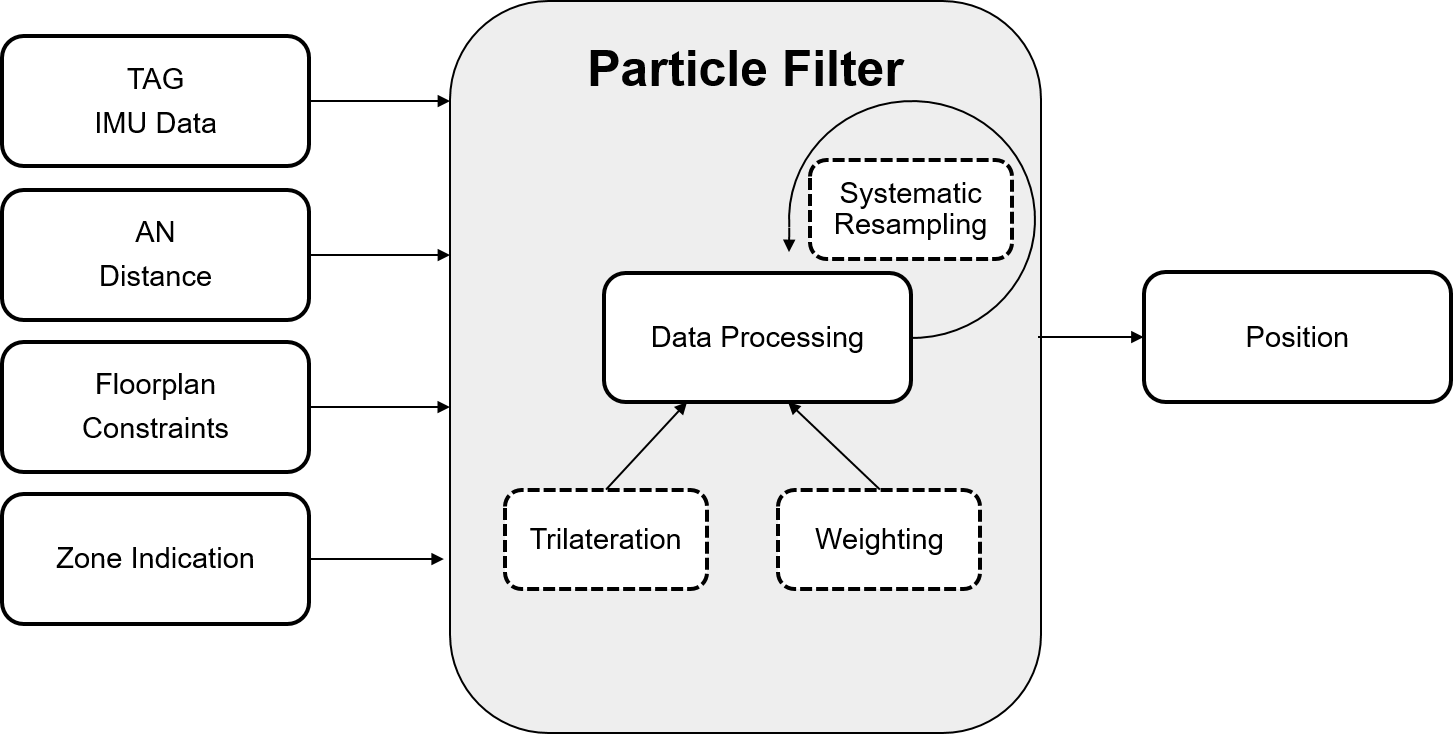
\includegraphics[width=1.0\textwidth]{Figures/particle_filter_design}
\decoRule
\caption[Particle Filter Design]{Overview of the theoretical components in our system.}
\label{fig:particle_filter_design}
\end{figure}


%----------------------------------------------------------------------------------------
%	SECTION 2
%----------------------------------------------------------------------------------------

\section{Setup}
The theoretical design of our system is shown in figure \ref{fig:system_design}, it works as follows:
At least three ANs, equipped with UWB technology, are placed in an indoor environment of one floor. Our algorithm runs on a seperate server, where a zoneplan and floorplan of the floor are available. A single TAG is located somewhere on the floor, it is as well equipped with UWB technology, moreover it measures acceleration and magnetic energy with the onboard IMU. The TAG continously collects data from the IMU and contemporary waits for a request from the server. The server periodically requests data via UWB from the TAG. As soon as a request is noticed at the TAG, it performs a range estimation to every AN and sends this data together with the continously collected IMU data to the server.
For every estimation period, the server has all the data needed to feed the particle filter.

\begin{figure}[th]
\centering
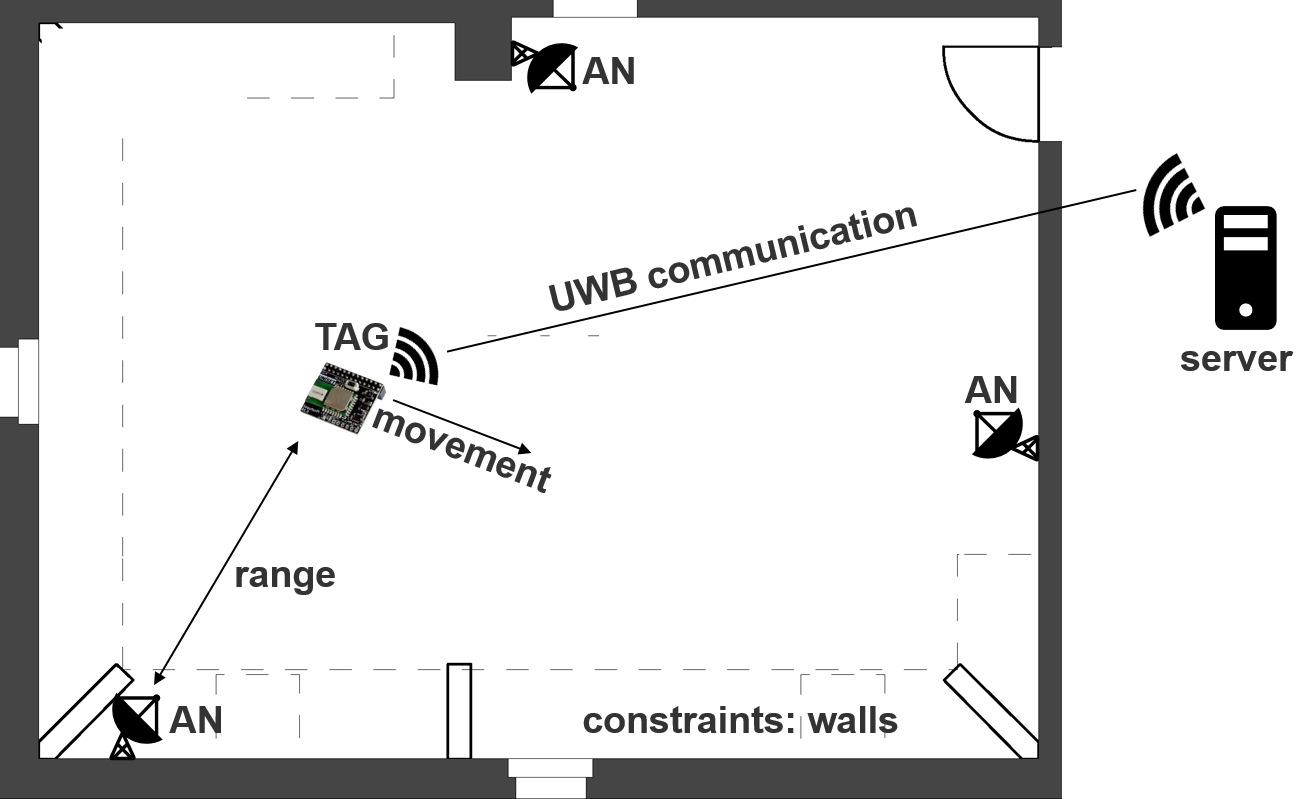
\includegraphics[width=1.0\textwidth]{Figures/system_design}
\decoRule
\caption[System Design]{Overview of the theoretical system design.}
\label{fig:system_design}
\end{figure}

%----------------------------------------------------------------------------------------
%	SECTION 3
%----------------------------------------------------------------------------------------

\section{Computations on the server}
Most computations are done on the seperate server, as we would like to minimize the required computational power and energy consumption of the devices. As already mentioned, the server receives IMU data and range estimations from the nodes. This data, as well as the floorplan constraints and the zone indication, flow into the particle filter. These operations are done on the server:
\begin{itemize}
\item Spread the particles and validate new positions with floormap constraints
\item Evaluate UWB ranges, IMU measures and zone indication to assign likelihood
\item Calculate weight function and systematically resample (and reposition) particles with low weights
\item Sum up weighted positions
\end{itemize}

In the first part, every particle is moved from its current to a new position. To validate the new position, we check if the direct trajectory between the old and the new location intersects with an impediment. If so, a new position is generated, as the last was not reachable.
The second item covers the likelihood of the new position. For every AN, the measured distance is compared to the distance from the new position to the AN. The less these two distances differ, the higher is the assigned liklihood. In this phase also the zone indication is taken into account. An AN that lies in the predicted zone is assumed to be more accurate than ANs far away, so the likelihood is even higher, when a near anchor has a small difference in range estimation. For the IMU motion, the difference between the old and the new positon is compared to the measured IMU motion to evaluate the likelihood.
In the weighting step, every particle gets weighted by the liklihoods of the previous computations. The weights of all particles are normalized for further processing.
The last part is simply a weighted sum of the particles locations.
% Chapter Template

\chapter{Implementation and experiment setup} % Main chapter title

\label{Chapter4} % Change X to a consecutive number; for referencing this chapter elsewhere, use \ref{ChapterX}
In this section we explain in detail, what hardware we used in our implementation and with which technology the UWB communication and ranging was done. Then we introduce the zone indication learning algorithm and finally we briefly explain the core of our work, the mathematical theory of the particle filter.

%----------------------------------------------------------------------------------------
%	SECTION 1
%----------------------------------------------------------------------------------------

\section{Hardware}
We decided to use Raspberry Pis for all mobile devices such as the TAG and the ANs. As the Raspberry Pis were not equipped with UWB technology, we extended them with a SEQUITUR Pi board from UNISET company running InGPS Lite firmware. In the following two subsections we present you these two hardware components.

%-----------------------------------
%	SUBSECTION 1
%-----------------------------------

\subsection{Raspberry Pi}
A Raspberry Pi is a single-board computer not much bigger than a credit card. Raspberry Pis are mainly designed for educational purposes as an alternative to expensive notebooks or desk computers. Hence the focus lies also on easy-to-use and plug-and-play experiences. Raspberry Pis are useful for versatile types of projects, as they provide common state of the art hardware - like HDMI, USB and wireless LAN - direct on boad and as they are extendable with selected components.

We used Raspberry Pi Model B \cite{Raspberry}, these were the most relevant specifications for our work:
\begin{itemize}
\item Quad Core 1.2GHz Broadcom BCM2837 64bit CPU
\item 1GB RAM
\item BCM43438 wireless LAN
\item 100 Base Ethernet
\item 40-pin extended general purpose input output (GPIO)
\item Micro SD port for loading your operating system and storing data
\end{itemize}

%-----------------------------------
%	SUBSECTION 2
%-----------------------------------
\subsection{SEQUITUR Pi board with InGPS Lite}
On the 40-pin extended GPIO, we connected the SEQUITUR Pi board from UNISET Company. UNISET is a company located in Italy that focuses on research, development and manufacturing of innovative sensors in two major application areas \cite{Uniset}:

\begin{itemize}
\item Access control security systems, enhancing the reliability of intrusion detection
\item Indoor and outdoor tracking. Sequitur is a precise real time locating system (RTLS) for tracking any object in 2D or 3D with centimeter accuracy.
\end{itemize}

This hardware seemed perfect for our ambitions, as it provides a state-of-the-art UWB communication and ranging. Moreover the SEQUITUR Pi board of the TAG has IMU sensors like 3D-accelerometer and 3D-magnetometer on board. Together with the hardware, UNISET delivers a firmware running on Raspberry Pis operating system (OS) to establish a connection via user datagram protocol (UDP). This firmware allows to communicate with the sensors in order to retrieve IMU sensor data, but also to get direct access to the range between two nodes. It is explained in detail throughout the next section. 

%----------------------------------------------------------------------------------------
%	SECTION 2
%----------------------------------------------------------------------------------------

\section{UWB Communication and Ranging}
The radio module of SEQUITUR Pi board is used on the one hand to transmit data - in order to obviate the need for additional communication hardware - and on the other hand to evaluate the ToF. As UNISET is a comercial company, they do not provide full information of the underlying transmission techniques. Nonetheless in the two following subsections, the known parts are mentioned.

%-----------------------------------
%	SUBSECTION 1
%-----------------------------------
\subsection{Transmission}
SEQUITUR InGPS Lite enables single-hop wireless communication with the UWB interface between neighboring nodes of the same network. 
The radio module supports six different user-selectable frequency bands between 3.5 GHz and 6.5 GHz. There are six different operation modes to change the spectral occupation, listed in the table below:\\
\\
\begin{tabular}{c c c}
Channel Number  & Central Frequency [MHz] & Bandwidth [MHz]\\
1 & 3494.4 & 500\\
2 & 3993.6 & 500\\
3 & 4492.8 & 500\\
4 & 3993.6 & 1300\\
5 & 6489.6 & 500\\
7 & 6489.6 & 1100\\
\end{tabular}
\\
\\
The data rate can be changed to three preset values of 110 kilobit per second (kbps), 850 kbps and 6.8 megabit per second (Mbps). All nodes have to operate in the same radiomode to communicate correctly. A lower data rate allows lager operating distances between the nodes. 
The default pulse repetition frequency (PRF) is assumed to 64 MHz for all the channels.
The underlying modulation techniques are not indicated in the specifications \cite{Usermanual} \cite{Beginnersguide}.

%-----------------------------------
%	SUBSECTION 2
%-----------------------------------
\subsection{Ranging with TWR}
UNISET company offers two different packages for positioning. InGPS Lite, which is the standard software and InGPS Pro, which is the advanced package. For our implementation InGPS Lite was sufficient, as the main difference of the two packages are the number of TAGs and anchors supported. With InGPS Lite only one TAG and a maximum of 10 anchors are supported as with InGPS Pro numerous TAGs and anchors are possible. InGPS Lite opperates only in TWR mode other than InGPS Pro, where a second mode with TDOA range estimation is available.
The range estimation of two nodes is triggered by the application programming interface (API) command $CLIENT\_GET\_RANGE\ (50)$. In our application we sent the command to the anchor in order to minimize the communication of the TAG. The flow of actions related to this API is a even more simplified version of the message exchange indicated in figure \ref{fig:two_way_ranging}. In our case, the request message performed by the client starts the TWR conversation via UWB between AN and TAG. The AN sends only one ranging request to the TAG, which immediately responds. By observing the difference between the time instants related to the transmission of the request packet and the reception of the response packet, the AN will directly determine the RTT and thus the range. Finally an answer message with the range is reported from the AN to the client and no messages are reported from the TAG to the client.


%----------------------------------------------------------------------------------------
%	SECTION 3
%----------------------------------------------------------------------------------------

\section{Zone Indication: Descriminative Ensemble Learning with Hidden Markov Models}
The zone indication is a rather complex and computationally demanding process, thus we will expain it to higher detail than the other inputs of the particle filter. The zone indication fuses Wi-Fi, UWB, magnetic field (MF) and room transition information in an enhanced learning model. A set of independent individual machine learning methods are combined in an ensemble learning model. The used approach integrates Hidden Markov Model (HMM) with discriminative learning techniques as presented in an earlier work of CDS \cite{Carrera2}.

%-----------------------------------
%	SUBSECTION 1
%-----------------------------------
\subsection{HMM-Discriminative Ensemble Learning Method}
In this approach different machine learning algorithms are combined to improve the zone prediction result. A zone can be defined as any subarea in the area of interest (e.g. a room). In the concept of Markov localization \cite{Markov}, the state of the system is estimated by the state transitions. For localization, the states of the model correspond to defined zones.
Therefore, the HMM is specified by the following components, as in \cite{Carrera2}:
\begin{itemize}
\item A set of $n$ states $Z=\{z_{1}, z_{2},\dots,z_{n}\}$, with $z_{i}$ as the identifier value of the zone $i$. Resulting the descrete random variable $x_{t} \in Z$ representing the hidden state at time t.
\item A quadratic matrix $A$ holding the transition probabilities,
\begin{equation*}
A = 
\begin{pmatrix}
   a_{1,1} & a_{1,2} & \dots & a_{1,n}\\
   a_{2,1} & a_{2,2} & \dots & a_{2,n}\\
    \vdots & \vdots & \ddots & \vdots  \\
   a_{n,1} & a_{n,2} & \dots & a_{n,n}\\
\end{pmatrix},
\end{equation*}
where $a_{ij}$ respresents the probability of moving from zone $z_{i}$ to zone $z_{j}$.
\item A set of observations O, defined as:
$$O = \{(o_{1},o_{2},\dots,o_{m})_1, \dots, (o_{1},o_{2},\dots,o_{m})_r\}$$
where $o_{i}$ stands for the zone prediction result of the $i$-th individual machine learning algorithm. This leads to $O$ being a set of $^rP_m$ permutations (repetitions allowed), with $r$ being the number of zones and $m$ the number of different machine learning algorithms. The machine learning methods have to be conditionally independent for $y_{t} \in O$ as the random variable of the observations in time $t$.
\item A matrix $B$ holding the emission probabilities of observation likelihoods:
\begin{equation*}
B = 
\begin{pmatrix}
   b_{1,1} & b_{1,2} & \dots & b_{1,r}\\
   b_{2,1} & b_{2,2} & \dots & b_{2,r}\\
    \vdots & \vdots & \ddots & \vdots  \\
   b_{n,1} & b_{n,2} & \dots & b_{n,r}\\
\end{pmatrix},
\end{equation*}
where $b_{ij}$ respresents the probability of $(o_{1},o_{2}, \dots, o_{m})_j$ being the observation generated in zone $z_{i}$.
\item An initial probability distribution $\pi = \pi_{1},\pi_{1},\dots, \pi_{n}$ over the $n$ zones.
\end{itemize}
How the specified components interact in the HMM can be seen in figure \ref{fig:hidden_markov_model}.


\begin{figure}[th]
\centering
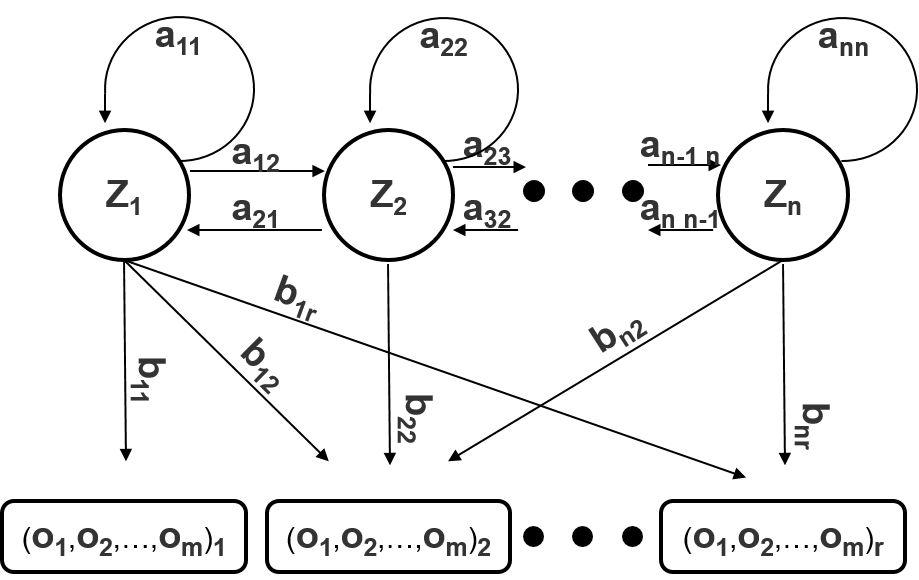
\includegraphics[width=0.8\textwidth]{Figures/hidden_markov_model}
\decoRule
\caption[HMM]{Application of the different probabilistic parameters in the hidden markov model.}
\label{fig:hidden_markov_model}
\end{figure}

The learning of each individual machine learning method only relies on the fingerprint of Wi-Fi, UWB and magnetic field, that's why prediction errors can still occur. However we can integrate the zone transition information (e.g. some areas are only reachable through other areas) in the HMM to improve the prediction. To determine the sequence of variables that is underlying source of some sequence of observation in a model with hidden variables, a decoding task is necessary. With the HMM model $\lambda = \{\pi, A, B\}$ and the given observation sequence $y_{t-i},\dots, y_{t-1},y_{t}$, the Viterbi algorithm \cite{Viterbi} is used to estimate the hidden states sequence $x_{t-i},\dots,x_{t-1},x_{t}$.

%-----------------------------------
%	SUBSECTION 2
%-----------------------------------
\subsection{Transition and Emission Probabilities in the HMM}
In advance, all zones are exactely defined. Then, the transition probabilies in matrix $A$ express the likelihood of moving from a beforehand defined zone to another. The connections between zones, retrieved from the floorplan, predetermine these probabilities. Therefore the values in the $n\times n$-matrix $A = (a_{ij})$ are defined as follows:
$$a_{ij} = P(x_{t+1} = z_{j} | x_{t} = z_{i})$$
where $a_{ij}$ represents the transition likelihood from zone $z_{i}$ to zone $z_{j}$. Thus, $\forall i \in \{1,\dots,n\}: \sum_{j=1}^{n} a_{ij} = 1$.\\
The emission probability is the likelihood of observing a particular set of observations $y_{j}$ at zone $z_{i}$. Therefore the values of the $n\times r$-matrix $B = (b_{ij})$ can be written as:
$$b_{ij} = P(y_{j} | z_{i}), \forall y_{j} \in O \land z_{i} \in Z,$$
where $y_{j} = (o_1, o_2, \dots, o_m)_j$ and $o_i$ is the zone prediction result from the $i$-th machine learning algorithm.
Since different individual machine learning methods are used independently, we can assume with good reason that their outcomes are conditionally independent. This leads to the simplified expression:
$$b_{ij} = \prod^{n}_{n=1} P(o_{j} | z_{i})_{n},$$
where $P(o_{j} | z_{i})_{n}$ is the probability of the $n$-th learning method predicting $o_{j}$ at zone $z_{i}$. Therefore it is equal to the sensitivity of the $n$-th machine learning algorithm at zone $z_{i}$:
$$P(o_{j} | z_{i})_{n} = \frac{TP_{n}}{TP_{n} + FN_{n}},$$
with $TP_{n}$ and $FP_{n}$ being the true positive respectively the false positive rate of the corresponding ML algorithm.
%also include the ML specification, (parameter and used methods) maybe in implementation?


%----------------------------------------------------------------------------------------
%	SECTION 4
%----------------------------------------------------------------------------------------

\section{Particle Filter}
We used a particle filter approach to solve the localization problem. This method, also known as Monte Carlo Localization (MCL), is often used for indoor positioning. It combines various noisy measurements to estimate the system state and minimize errors. To introduce the particle filter, we explain in a first paragraph which inputs we fused into the particle filter. The following paragraphs define the different phases in our mathematical model whereas we discuss the different variations of our system in the last subsection.

%-----------------------------------
%	SUBSECTION 1
%-----------------------------------
\subsection{Inputs}
As stated above, various measurements are taken into account in our particle filter. The most important inputs are the range estimations between the TAG and ANs, the motion vector measured by the IMU of the TAG and the restrictions given by the floormap. We will refer to $Zd_{t}$ as the range observation vector at time t, which is described as $Zd_{t} = [d^{j}_{t}], j = 1...N,$ where N is the number of ANs. Every distance measurement $d^{j}_{t}$ itself is consisting of various errors, statistically it can be described as: 
$$d^{j}_{t} = \hat{d}^{j}_{t} + d^{j}_{be, t} + \epsilon_{d^{j}, t},$$
where $\hat{d}^{j}_{t}$ is the actual distance to node j, $d^{j}_{be, t}$ is an environmental bias due to local conditions (obstacles) and $\epsilon_{d^{j}, t},$ is a measured random error.

The motion vector $Mv_{t} = [\theta_{t}, \ell_{t}]$ is modeled by the heading direction $\theta$ and the movement length $\ell$. Both of $\theta$ and $\ell$ are calculated by the IMU readings, where again several noises occur such that the heading direction is statistically described as:
$$\theta_{t} = \hat{\theta}_{t} + \theta_{bs,t} + \theta_{be,t} + \epsilon_{\theta, t},$$
with $\hat{\theta}_{t}$ as the actual heading orientation,  $\theta_{bs,t}$ as a sensor bias introduced by uncalibrated sensor readings, $\theta_{be,t}$ as an environmental angular bias due to magnetic field disturbances and $\epsilon_{\theta, t}$ as a measured random error. 
In our implementation we calculated the heading direction with the formula $\theta = atan(\frac{mag_{x}}{mag_{y}})$, where $mag_{x}$ and $mag_{y}$ are low pass filtered magnetometer readings in x and y direction. The update frequency of the sensor was higher than the update frequency of the particle filter, hence we calculated an average of these different measurements, hereafter appearing as $\theta_{t}$ for the average during time period from t-1 to t.

Whereas the heading direction is directly calculated from IMU data, for the stride length we took the previous system state into account. This was necessary, because measured errors propagate over time, so it is almost impossible to use relative quantities (e.g. acceleration) to calculate absolute quantities (e.g. distance) over a longer period of time. As we can not assume the acceleration to be constant, the movement length approximation can be defined as: 
$$\ell_{t} = \hat{\ell}_{t-1} + \sum_{i=0}^{N}([(\hat{a}_{i} + a_{bs,i} +\epsilon_{a, i}) * \Delta t_{i} ]*(N-i)) *\Delta t + \epsilon_{\ell, t},$$
where $\hat{\ell}_{t-1}$ is the actual movement length of time period t-1, $\hat{a}_{i}$ is the actual middle acceleration during the $i$-th of N time slots in time period $\Delta t$, $a_{bs,i}$ is an other sensor bias due to uncalibrated sensor readings and $\epsilon_{a, i}$ as well as $\epsilon_{\ell, t}$ are measured random errors in acceleration and distance respectively.
In our implementation the observed movement length is calculated as follows:
$$\ell_{t} = v_{t-1} * \Delta t + \sum_{i=0}^N [(a_{i} * \Delta t_{i})(N-i)]* \Delta t$$
where $v_{t-1}$ is the velocity of the estimated position change in the last system state update, $a_{i}$ is the $i$-th acceleration measurement and N the number of descrete acceleration measurements during the time period $\Delta t$, which corresponds to the time passed between t-1 and t. As the acceleration sensor - depending on pitch and roll of the device - had a huge non-zero mean noise, we decided to not use the accelerometer data directly, but to use the change in acceleration. To gather the change in acceleration we fed the sensor data into two low pass filters with different parameters, one with a high adaption and one with a low adaption, and only took their difference into account. This corrects a part of the long term sensor bias. 

Although there were many sources of errors, for the likelihood calculation in our work we nevertheless used the actual obtained values $d^{j}_{t}$, $\theta_{t}$ and $\ell_{t}$ since the errors are handled in the likelihood model by fusing different data sources and anchor node distances. However, to compensate the bias and error for the particle spreading, we assumed the heading direction $\theta$ and the stride length $\ell$ as random normal variables whose values are obtained from $\mathcal{N}(\theta_{t}, \sigma_{\theta}^{2})$ and $\mathcal{N}(\ell_{t}, \sigma_{\ell}^{2})$.

%-----------------------------------
%	SUBSECTION 2
%-----------------------------------
\subsection{Prediction phase}
Each particle has a state vector that is defined as follows:
$$X_{t} = [x_{t}, y_{t}, x_{t-1}, y_{t-1}]$$
where $(x_{t}, y_{t})$ corresponds to the Cartesian coordinates of the particle at time t and $(x_{t-1}, y_{t-1})$ at time t-1 respectively. In the prediction phase each particle is updated depending of the current movement vector $Mv_{t} = [\theta_{t}, \ell_{t}]$. The coordinates of the particle are updated with the following pattern:
$$[x_{t}, y_{t}]  = [x_{t-1} + \ell_{t} * cos(\theta_{t}),\quad y_{t-1} + \ell_{t} * sin(\theta_{t})]$$
As mentioned in the last subsection, with $\ell_{t}$ and $\theta_{t}$ as random normal variables. In the remainder of this work we will also refer to the motion in Cartesian coordinates as $M_{x,t} = \ell_{t} * cos(\theta_{t})$ for the motion in x-direction and $M_{y,t} = \ell_{t} * sin(\theta_{t})$ for the motion in y-direction.
Floorplan restrictions are applied in this phase, whereas movements through walls are not permitted, they lead to another prediction iteration for that particle.

%-----------------------------------
%	SUBSECTION 3
%-----------------------------------
\subsection{Observation phase}
In the observation phase an associated weight $w^{i}_{t}$ is recalculated for every particle, since the weight does not anymore correspond to the current position. The weight is updated corresponding to the likelihood of the range observations conditioned on each particle $p(Zd_{t} | X^{i}_{t})$ at time t, respectively the likelihood of the motion observation conditioned on each particle $p(Mv_{t} | X^{i}_{t})$ at time t. Then, the probability is determined as:
$$ p(Zd_{t} | X^{i}_{t}) = p(d_{t}^{j} | X^{i}_{t}) $$
and $$ p(Mv_{t} | X^{i}_{t}) = p(M_{x,t} | X^{i}_{t}) * p(M_{y,t} | X^{i}_{t}).$$ %is this correct that p(x) and p(y) are multiplied?
In addition, as defined in subsection 4.3, the zone probability is:
$$ p(y_t | X^{i}_{t}) = p(y_{t} | z^{i}_{t})$$
where $y_t$ is the observed fingerprint at time $t$ and $z^{i}_{t}$ the current zone of particle $X^{i}$.
In order to avoid confusion between different likelihoods used in this work, hereafter we refer to $p(d_{t} | X^{i}_{t})$ as the ranging likelihood, $p(M_{t} | X^{i}_{t})$ for the motion likelihood, $p(y_t | X^{i}_{t})$ for the zone likelihood and $p(Z_{t} | X^{i}_{t})$ as the overall likelihood.

The associated weight $w^{i}_{t}$ of each particle is given by ranging as well as by motion information. A particle at the current position $(x_{t},y_{t})$ with low probability to observe $d_{t}^{j}$ in its position will be assigned a small weight. Additionally a particle that moved in x-direction by $x_{t}^{i}-x_{t-1}^{i}$ with low probability to observe the movement $M_{x,t}$ will also be assigned a small weight. Analogue for the movement in y-direction.
That leads to the fact that particles with large weights will have a stronger effect to the determination of the state of the system.
We assume that all these likelihoods - the ranges to each AN as well as the movement in direction x, y - are statistically independent from each other. Therefore, the overall likelihood is defined as:
$$p(Z_{t} | X^{i}_{t}) = \prod_{j=1}^{N} p(\hat{d}_{j,t}|X_{t}^{i}) * p(\hat{M}_{x,t} | X^{i}_{t}) * p(\hat{M}_{y,t} | X^{i}_{t}) * p(y_t | X^{i}_{t})$$
where $\hat{d}_{j,t}$ is the measured distance to the AN j at time t and $\hat{M}_{x,t}$ is the measured motion in x-direction in timeinterval t, respectively $\hat{M}_{y,t}$ in y-direction and $y_t$ is the measured RSS fingerprint.

The individual likelihood for the range observation can then be expressed as:
$$p(\hat{d}_{j,t} | X^{i}_{t}) = \frac{1}{\sqrt{2\pi \sigma_{j}^{2}}} * exp(\frac{-[\sqrt{(x^{i}_{t}-x_{j})^{2}+(y^{i}_{t}-y_{j})^{2}} - \hat{d}_{j,t}]^{2}}{2\sigma_{j}^{2}})$$
where $(x_{j},y_{j})$ are the known coordinates of the $j$-th AN.
Whereas the individual likelihood of the motion observation in x-direction (analogue for y-direction) is expressed as follows:
$$p(\hat{M}_{x,t} | X^{i}_{t}) = \frac{1}{2\pi \sigma_{Mx}^{2}} * exp(\frac{-[(x^{i}_{t}-x^{i}_{t-1}) - \hat{M}_{x,t}]^{2}}{2\sigma_{Mx}^{2}})$$

%-----------------------------------
%	SUBSECTION 4
%-----------------------------------
\subsection{Resampling phase}
The resampling phase is an essential component of our particle filter implementation, although it is a computationally expensive step. In the resampling, particles with low assigned weights are repositioned at identical positions as particles with high associated weights. This means, that after the repositioning of the prediction phase and the weight calculation in the observation phase, a resampling in systematic manner is done. This resampling relies on the overall likelihood $p(Z_{t} | X^{i}_{t})$, which means that every kind of likelihood is taken into account for this step. After repositioning the particles with low weights (and updating their weight), all weights are normalized to obtain in the next step the weighted center of all particles, which corresponds to the estimated position. 
%-----------------------------------
%	SUBSECTION 5
%-----------------------------------
\subsection{Variants}
We implemented two variants of the particle filter localization system to state the effect on accuracy of the different parts in our system.
Hereafter we will refer to $PF_{full}$ for the full implementation of the particle filter as defined in the last subsection. However, the particles were not spread according to the movement vector, but randomly spread in a box of $2 \times 2$ meters centered on the last estimated position. We decided to cancel the movement vector for spreading, as it caused a very bouncy position estimation.
The second variant $PF_{UWBonly}$ is exclusively using UWB ranging and does not take the IMU measured movement or the fingerprint into account, neither in the prediction phase nor in the observation phase. 


%----------------------------------------------------------------------------------------
%	SECTION 5
%----------------------------------------------------------------------------------------

\section{Experiment Setup and parameter}
In our experiment we tested the localization accuracy of the different implemented variants, as well as the accuracy of the indoor tracking system UNISET company provided with their sensors, in a complex indoor scenario with trajectories through numerous of rooms on one floor in a real building of the University of Bern. During our experiments an additional test setup with optimized anchor node positions was defined.

%-----------------------------------
%	SUBSECTION 1
%-----------------------------------
\subsection{Zone indication: concrete implementation and parameter}
In our implementation these three completely different ML algorithms were used: KStar \cite{KStar}, Multilayer Perceptron (MLP) \cite{MLP} and the J48 decision tree \cite{J48}.  \textbf{ADAPT to GINI, SV and KNN}
The internal parameter of the ML algorithms were optimized from training data, whereas the following parameter were used for the non self optimizing parameters: global percent ratio of 30\% for KStar, single hidden layer with 10 neurons for MLP and a confidence factor of 0.25 for J48.
The zone definition can be seen in figure \ref{fig:zone_definition}.

We assumed that the liklihood of staying in the same zone is bigger than moving to another zone, which led to the empirically defined values for matrix $A$ as:

\begin{figure}[th]
\centering
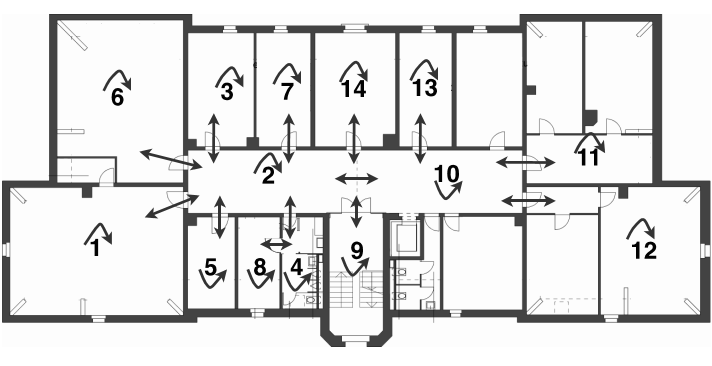
\includegraphics[width=1.0\textwidth]{Figures/zone_definition}
\decoRule
\caption[Zone Definition]{Zone definition and transitions between zones}
\label{fig:zone_definition}
\end{figure}

\textbf{MATRIX A has to be updated by the correct values}

\setcounter{MaxMatrixCols}{15}
\begin{equation*}
A = 
\begin{pmatrix}
0.6 & 0.4 & 0 & 0 & 0 & 0 & 0 & 0 & 0 & 0 & 0 & 0 & 0 & 0\cr
0.6 & 0.4 & 0 & 0 & 0 & 0 & 0 & 0 & 0 & 0 & 0 & 0 & 0 & 0\cr
0.6 & 0.4 & 0 & 0 & 0 & 0 & 0 & 0 & 0 & 0 & 0 & 0 & 0 & 0\cr
0.6 & 0.4 & 0 & 0 & 0 & 0 & 0 & 0 & 0 & 0 & 0 & 0 & 0 & 0\cr
0.6 & 0.4 & 0 & 0 & 0 & 0 & 0 & 0 & 0 & 0 & 0 & 0 & 0 & 0\cr
0.6 & 0.4 & 0 & 0 & 0 & 0 & 0 & 0 & 0 & 0 & 0 & 0 & 0 & 0\cr
0.6 & 0.4 & 0 & 0 & 0 & 0 & 0 & 0 & 0 & 0 & 0 & 0 & 0 & 0\cr
0.6 & 0.4 & 0 & 0 & 0 & 0 & 0 & 0 & 0 & 0 & 0 & 0 & 0 & 0\cr
0.6 & 0.4 & 0 & 0 & 0 & 0 & 0 & 0 & 0 & 0 & 0 & 0 & 0 & 0\cr
0.6 & 0.4 & 0 & 0 & 0 & 0 & 0 & 0 & 0 & 0 & 0 & 0 & 0 & 0\cr
0.6 & 0.4 & 0 & 0 & 0 & 0 & 0 & 0 & 0 & 0 & 0 & 0 & 0 & 0\cr
0.6 & 0.4 & 0 & 0 & 0 & 0 & 0 & 0 & 0 & 0 & 0 & 0 & 0 & 0\cr
0.6 & 0.4 & 0 & 0 & 0 & 0 & 0 & 0 & 0 & 0 & 0 & 0 & 0 & 0\cr
0.6 & 0.4 & 0 & 0 & 0 & 0 & 0 & 0 & 0 & 0 & 0 & 0 & 0 & 0\cr
\end{pmatrix},
\end{equation*}

%-----------------------------------
%	SUBSECTION 2
%-----------------------------------
\subsection{Placement, trajectories and configuration}
We distributed the UWB anchor nodes over several rooms to cover the area of interest homogenously. The exact position is indicated in the floor plan of figure \ref{fig:anchor_position}. Whereas the particle filter updated its state every 700 milliseconds, the IMU sensors were updated every 100 milliseconds. The UWB transmitter of the TAG and the ANs operated in radio mode 2 with a datarate of 850 kbps, they were configured to use channel 4 with a central frequency of 3993.6 MHz and an occupied sprectrum of 1300 MHz.

\begin{figure}[th]
\centering
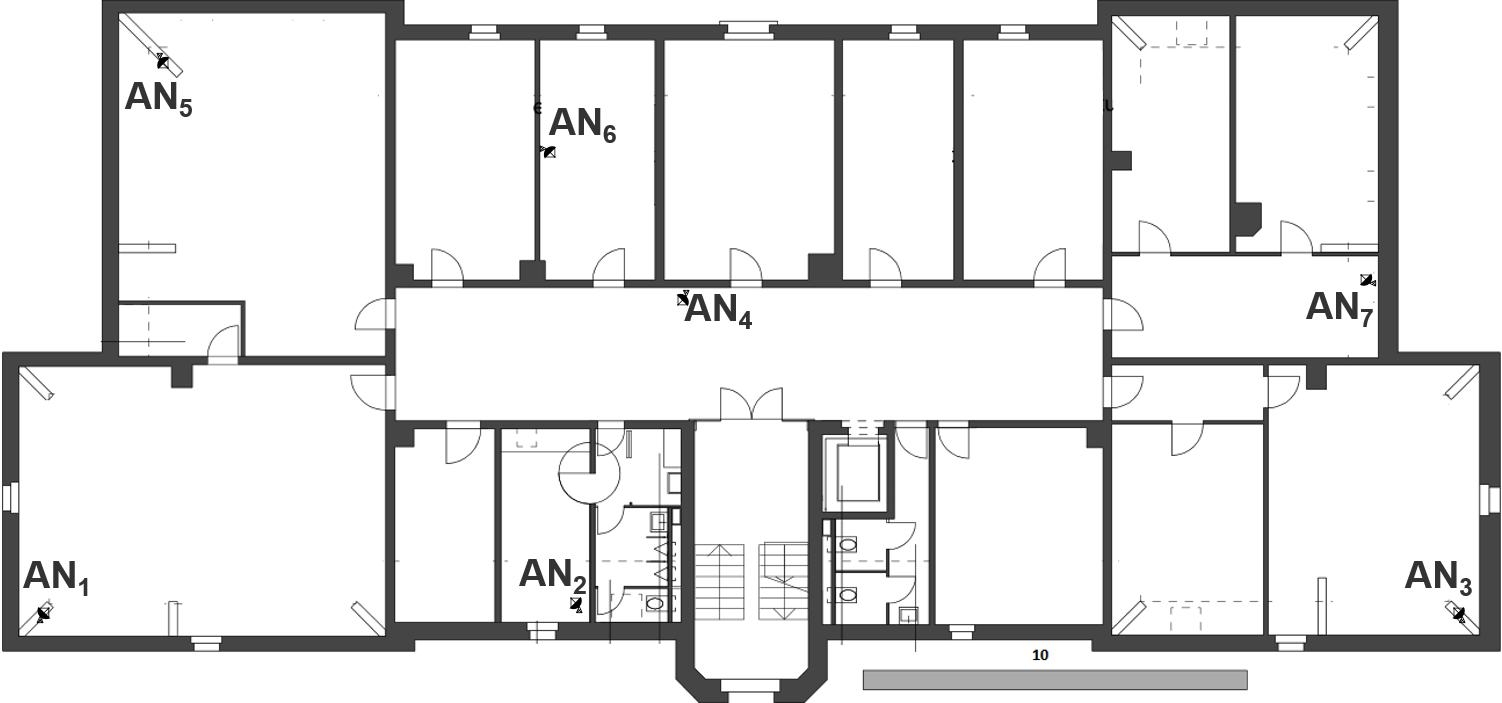
\includegraphics[width=0.8\textwidth]{Figures/anchor_position}
\decoRule
\caption[Anchor Node Positions]{Distributed anchor nodes on the floor map (with distance reference of 10m).}
\label{fig:anchor_position}
\end{figure}

The TAG was hold in the hand of a pedestrian at the starting point of the trajectories, when the experiments started. The pedestrian walked along the given path indicated in figure \ref{fig:trajectory1}, as soon as he passed a predefined checkpoint the current position estimation was registered. The other three trajectories can be seen in appendix \ref{AppendixA}. Every trajectory was tested with every algorithm 4 times.

\begin{figure}[th]
\centering
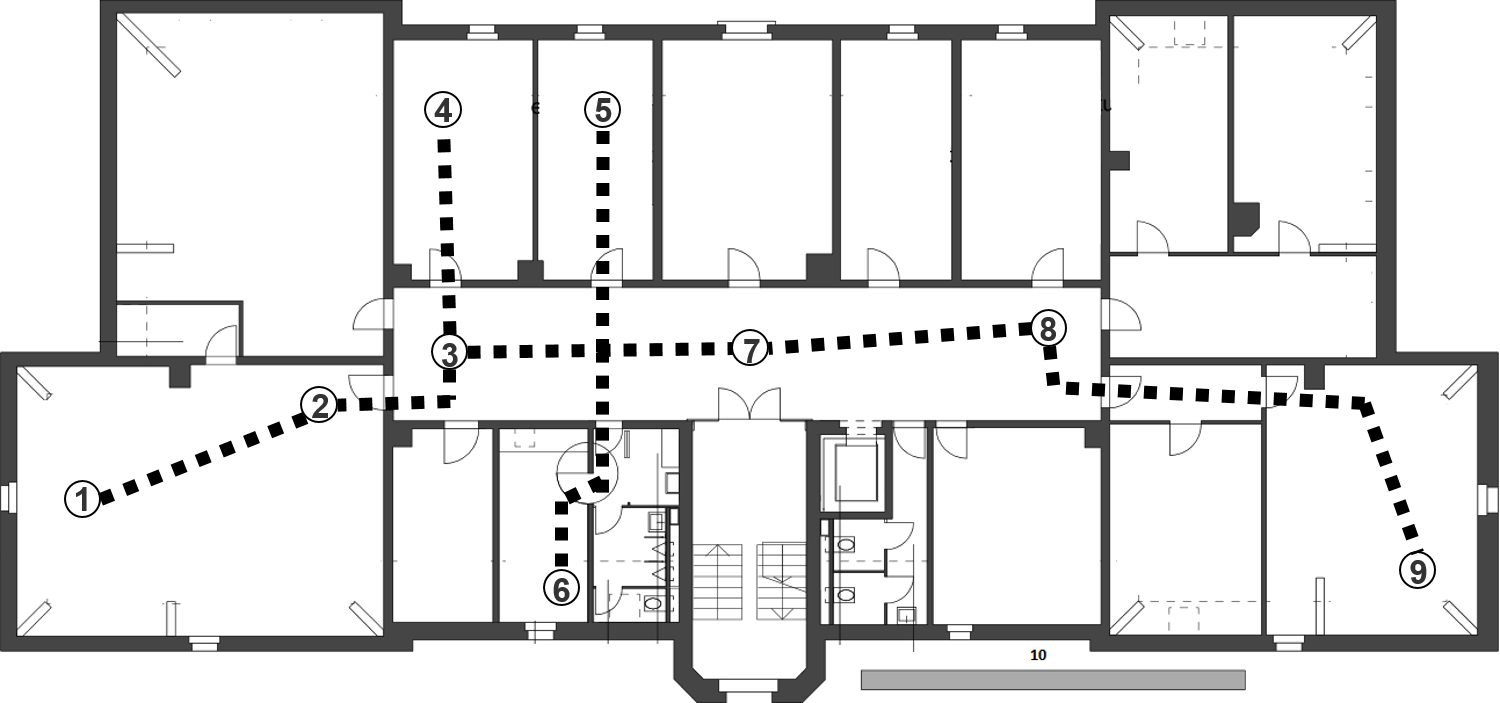
\includegraphics[width=0.8\textwidth]{Figures/trajectory1}
\decoRule
\caption[Trajectory 1]{Trajectory 1 of the four defined trajectories with the position checkpoints.}
\label{fig:trajectory1}
\end{figure}

In an ajusted experiment setup with improved anchor node positions we evaluated a fifth trajectory for every of the three algorithms. We just replaced the AN positions and did not change any other parameter. The new positions of the anchors and the trajectory checkpoints can be seen in figure \ref{fig:trajectory5_withAnchors}.

\begin{figure}[th]
\centering
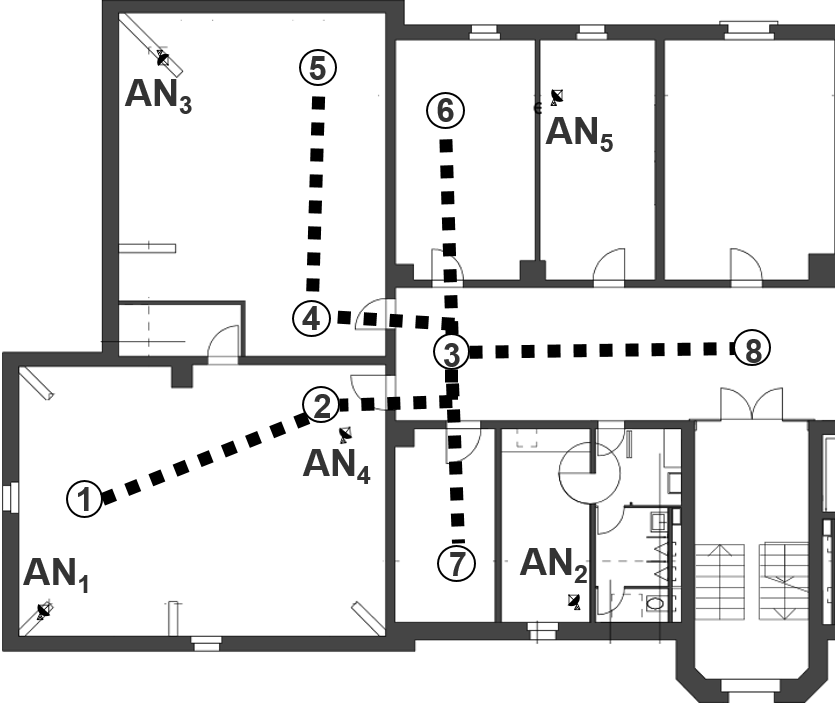
\includegraphics[width=0.5\textwidth]{Figures/trajectory5_withAnchors}
\decoRule
\caption[Trajectory 5]{Trajectory 5 with improved anchor positions.}
\label{fig:trajectory5_withAnchors}
\end{figure}
 
% Chapter Template

\chapter{Performance Evaluation} % Main chapter title

\label{Chapter5} % Change X to a consecutive number; for referencing this chapter elsewhere, use \ref{ChapterX}
In this section, we explain the setup of our two experiment scenarios and we present the positioning results of our experiments in detail.

%----------------------------------------------------------------------------------------
%	SECTION 1
%----------------------------------------------------------------------------------------

\section{Experiment Setup}
We tested our implementation in two complex indoor scenarios with trajectories through numerous rooms on one floor in a real building of the University of Bern, at Neubrückstrasse 10 in
3012 Bern. The first scenario used an area of $715m^2$ and the second scenario $358m^2$. We distributed the UWB anchor nodes over several rooms to cover the area of interest homogenously.
\begin{figure}[th]
\centering
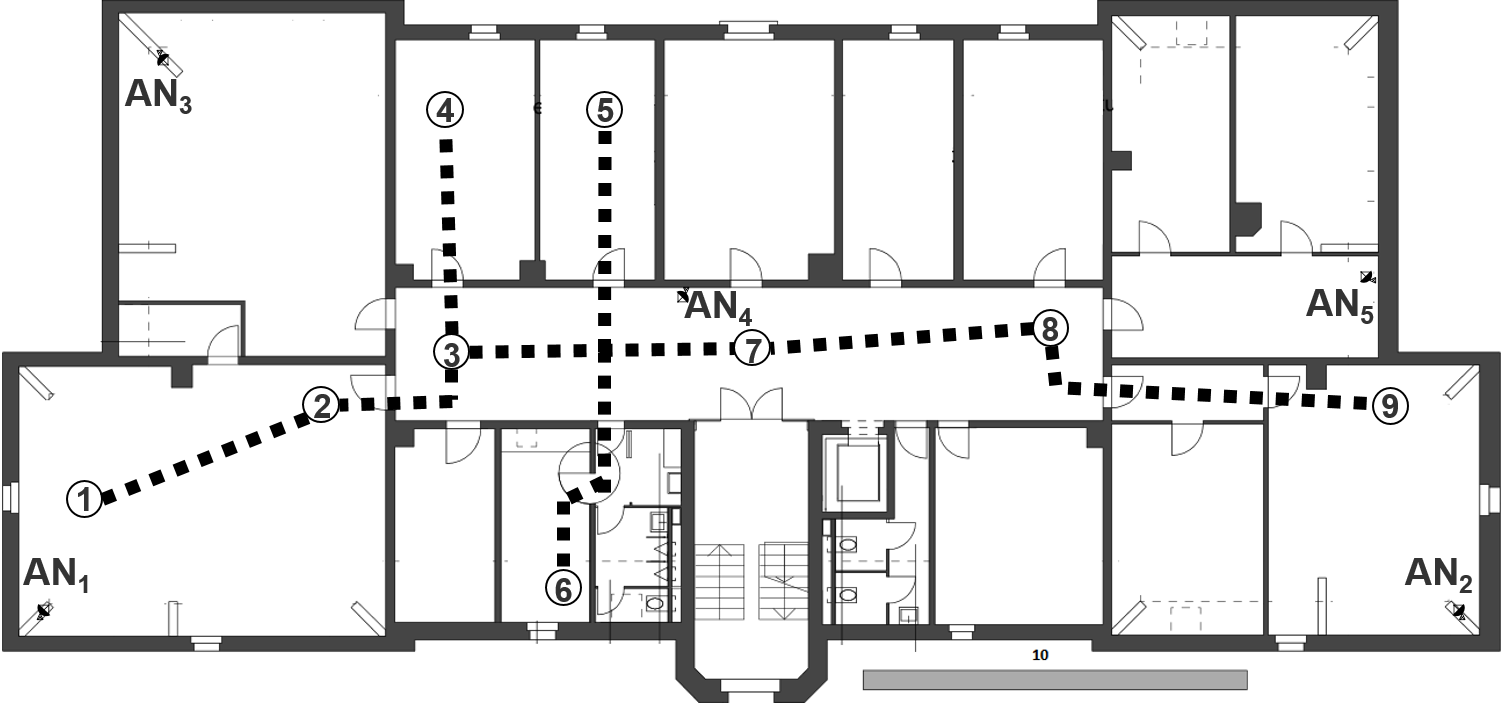
\includegraphics[width=0.8\textwidth]{Figures/trajectory1_withAnchors}
\decoRule
\caption[Anchor Node Positions of Scenario 1]{Trajectory 1 and distributed ANs in scenario 1 on the floor map (with distance reference of 10m).}
\label{fig:trajectory1_withAnchors}
\end{figure}The exact position is indicated in the floor plan of Figure \ref{fig:trajectory1_withAnchors} for the first scenario and indicated in Figure \ref{fig:trajectory5_withAnchors} for the second scenario. In both scenarios, the target was held in the hand of a pedestrian at the starting point of the trajectories, when the experiments started. The pedestrian walked along the given trajectory path. As soon as he passed a predefined checkpoint the current position estimation was registered.\\
\noindent\hspace*{5mm}%
We defined four different trajectories for the first scenario. Each trajectory consisted of five to nine checkpoints. Trajectory 1 is indicated in Figure \ref{fig:trajectory1_withAnchors}, the other three trajectories can be seen in Appendix \ref{AppendixA}.
For the second scenario we used a fifth trajectory that covered almost the whole area. It is shown in Figure \ref{fig:trajectory5_withAnchors}.\\
\noindent\hspace*{5mm}%
We repeated the experiment five times, so we analyzed 145 checkpoints in scenario 1 and 40 checkpoints in scenario 2.\begin{figure}[th]
\centering
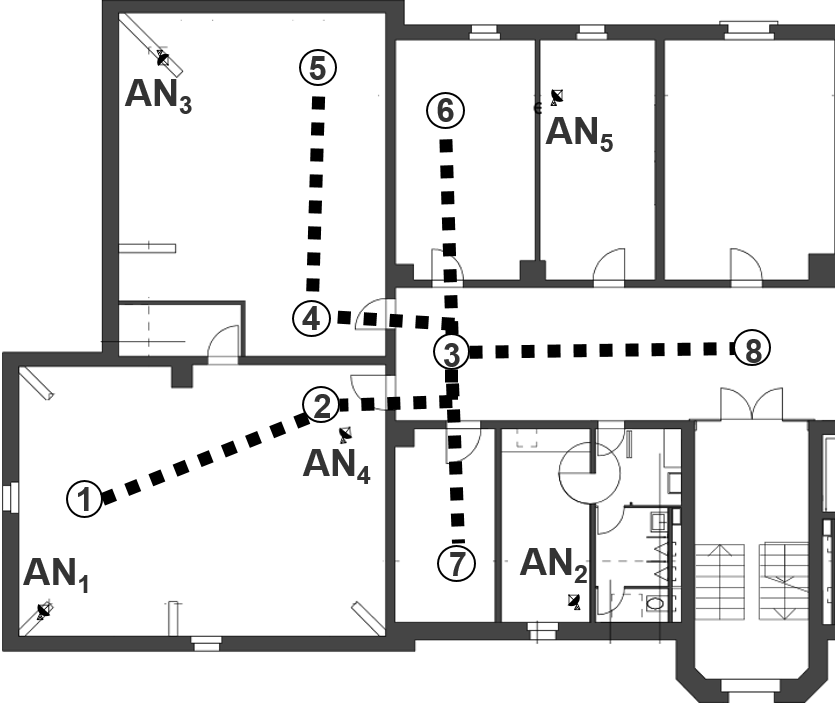
\includegraphics[width=0.5\textwidth]{Figures/trajectory5_withAnchors}
\decoRule
\caption[Trajectory 5]{Trajectory 5 with improved anchor positions.}
\label{fig:trajectory5_withAnchors}
\end{figure}
The localization error was determined by the Euclidian distance between the systems position estimation and the real position of the checkpoint.\\
\noindent\hspace*{5mm}%
For the zone detection in our algorithm, we defined 14 zones, which corresponded to 13 different rooms, where only one room (the corridor) was split into two zones. The room definitions can be seen in Figure \ref{fig:zone_definition}. For scenario 1 we collected data in all zones, whereas for the smaller scenario we only collected data in rooms 1, 2, 3, 5, 6 and 7, as only these were in the area of interest. The received signal strength values of all five UWB ANs as well as of eight Wi-Fi access points were taken into account. In order to reduce errors introduced by changing environmental conditions, we used relative RSS rather than raw RSS values. This means, we defined a pivot AN and access point and fed the machine learning algorithms with RSS difference to these given pivot RSS values and not the directly measured RSS values. In our scenarios, the AN 4 and the neighboring WiFi access point 8 were acting as a pivot (see Figure \ref{fig:trajectory1_withAnchors} and Figure \ref{fig:wifi_accessAppendix} for the exact positions). In the offline phase, we collected around 700 fingerprint measures per room. Half of them were collected randomly passing the room and half of them were collected while systematically walking through the whole area of the room.
\begin{figure}[th]
\centering
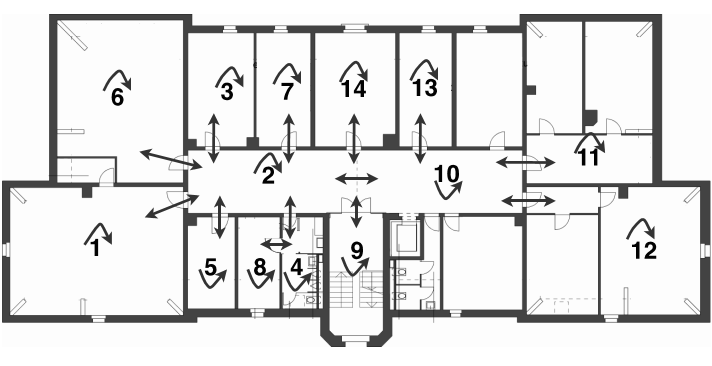
\includegraphics[width=1.0\textwidth]{Figures/zone_definition}
\decoRule
\caption[Zone Definition]{Zone definition and transitions between zones}
\label{fig:zone_definition}
\end{figure}

\section{Experiment Results}
Experiments were first conducted in scenario 1, then we covered a smaller area with a higher density of anchor nodes and conducted the experiments in scenario 2. As a reference, we compared our localization approach to a commercial localization system proposed by UNISET, called Sequitur InGPS Lite. In the following, we compare our particle filter results to the Sequitur system results.
\subsection{Localization Performance in Scenario 1}
In the following, the results of our algorithms with a wide distance between anchor nodes are shown. We called this setup scenario 1. Scenario 1 consisted of the wide anchor node positioning indicated in Figure \ref{fig:trajectory1_withAnchors}. In scenario 1 we tested four different trajectories, the trajectories 1-4. Trajectory 1 is indicated in Figure \ref{fig:trajectory1_withAnchors}, the trajectories 2, 3 and 4 are shown in Figure \ref{fig:trajectories2to4}.
\begin{figure}[th]
\centering
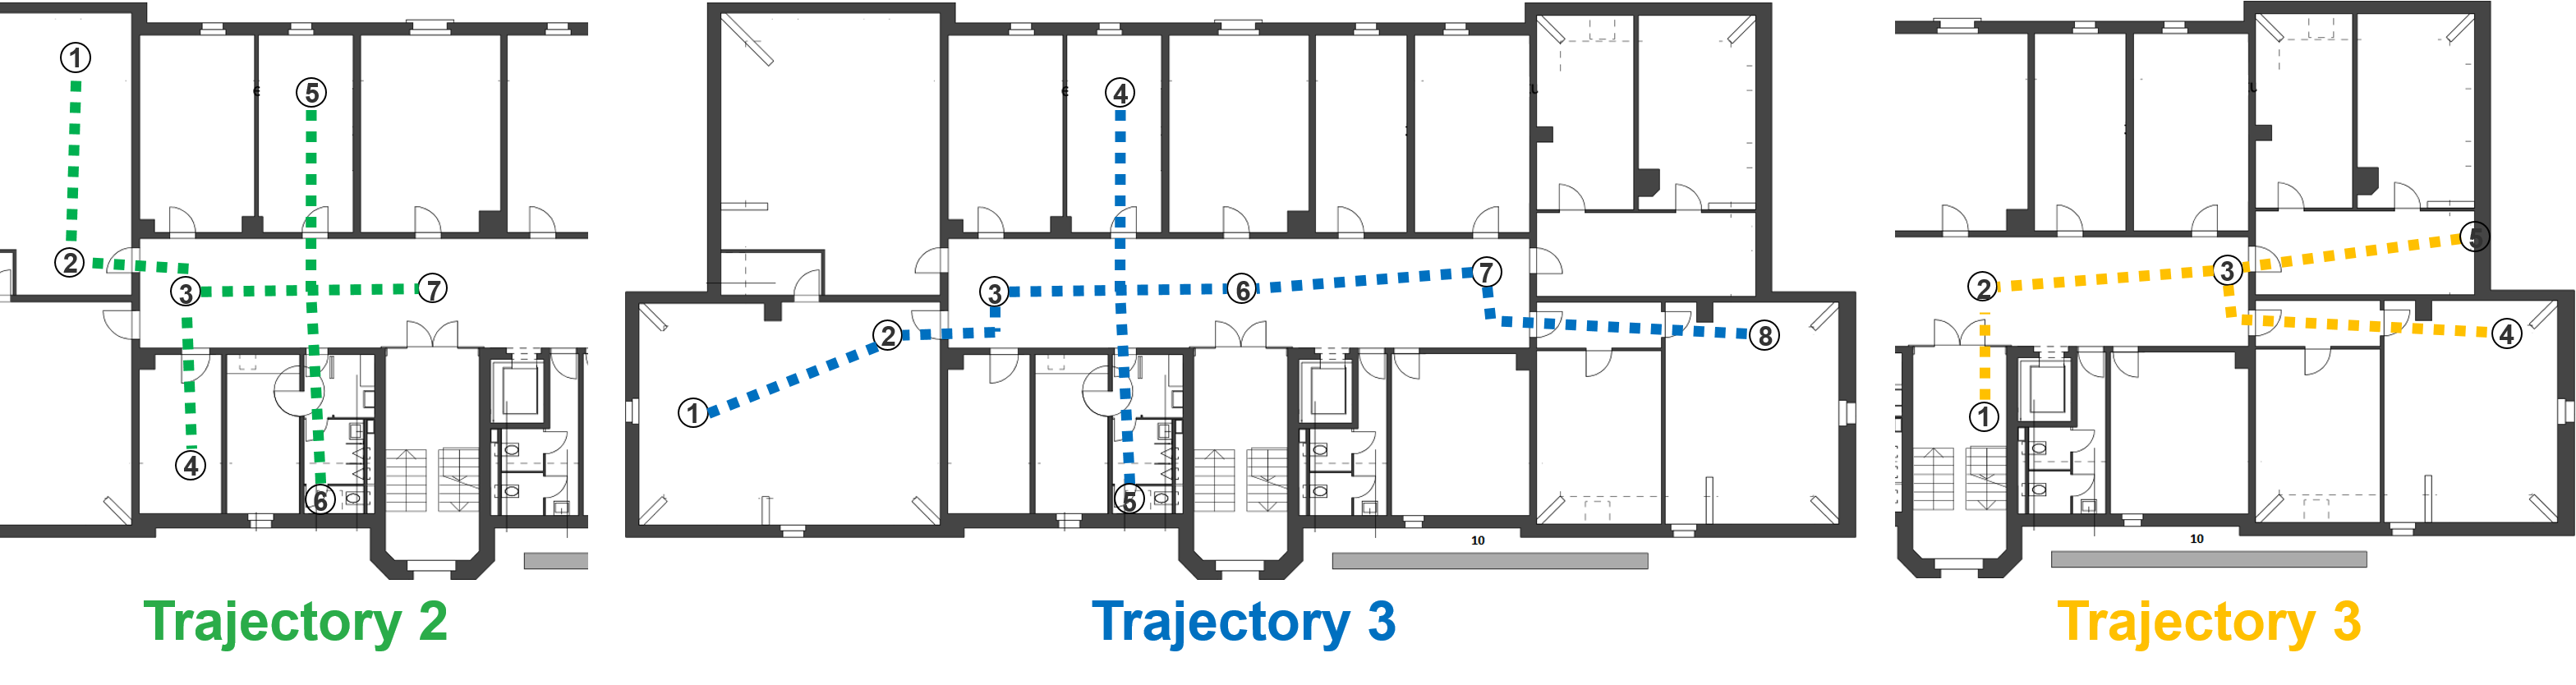
\includegraphics[width=1.0\textwidth]{Figures/trajectories2to4}
\decoRule
\caption[Trajectories 2-4]{Checkpoint position in Trajectories 2, 3 and 4}
\label{fig:trajectories2to4}
\end{figure}
The results are shown as arithmetic means of the five probes we registered.\\
\noindent\hspace*{5mm}%
In the first trajectory, the arithmetic mean (hereafter often called average) distance error over all checkpoints was $1.62$m for the particle filter and $1.75$m for Sequitur's commercial system. Looking at Figure \ref{fig:trajectory1and2_results}, we see that the errors are often smaller than $1.5m$, however, there are some checkpoints (e.g. checkpoint 5 in trajectory 1) with very low accuracy. This is also emphasized by comparing the arithmetic mean error to the median error of $1.12m$ for PF and $1.13m$ for Sequitur. The median errors are significantly lower than the arithmetic mean errors. The measurements for trajectory two looked rather similar but with a higher error. The arithmetic mean error for the PF was $2.39m$ and for Sequitur $2.35m$. The median errors were again a lot more accurate with $1.59m$ for PF and $1.16m$ for Sequitur.
\begin{figure}[th]
\centering
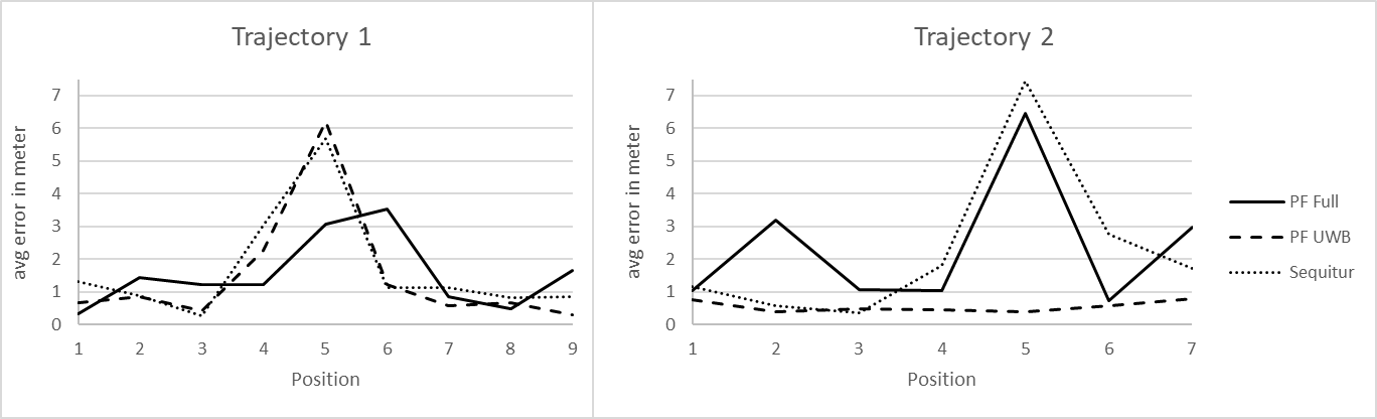
\includegraphics[width=1.0\textwidth]{Figures/trajectory1_2_results}
\decoRule
\caption[Localization Results of Trajectory 1 and 2]{Measured distance errors at each checkpoint in trajectory 1 and 2.}
\label{fig:trajectory1and2_results}
\end{figure}
The results for trajectory 3 and 4 were rather similar, however, the peaks observed in Figure \ref{fig:trajectory3and4_results} were not as extreme as for the first two trajectories. As above, the average errors in the third trajectory of $1.23m$ (PF) and $1.94m$ (Sequitur) were also considerably higher than the medians of $0.95m$ and $0.80m$.
\begin{figure}[th]
\centering
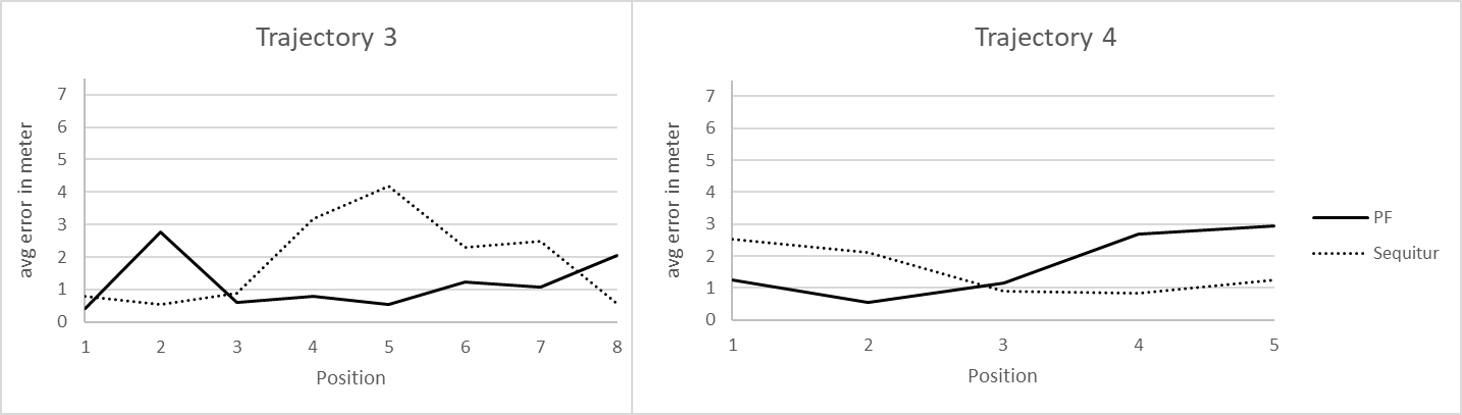
\includegraphics[width=1.0\textwidth]{Figures/trajectory3_4_results}
\decoRule
\caption[Localization Results of Trajectory 3 and 4]{Measured distance errors at each checkpoint in trajectory 3 and 4.}
\label{fig:trajectory3and4_results}
\end{figure}In the last of these four trajectories, no big outliers were stated. Nonetheless, the average errors of $1.79m$ and $1.55m$, as well as the median errors $1.24m$ and $1.26m$ for the PF and Sequitur, were still not as accurate as intended.\\
\noindent\hspace*{5mm}%
Having a closer look at table \ref{tab:arithmetic_errors}, we see that there are very big differences between different trajectories. The particle filter and the Sequitur system have similar accuracies, for some trajectories, one of the algorithms is better, for other trajectories the other performs better. Possible reasons for these volatile results are discussed in the upcoming subsection  \ref{Section2} about result analysis. 

\begin{table}
\caption{Arithmetic Mean of Errors in Trajectories 1 to 4 (meter).}
\label{tab:arithmetic_errors}
\centering
\begin{tabular}{l l l}
\toprule
\textbf{Trajectory} & \textbf{PF} & \textbf{Sequitur}\\
\midrule
\textbf{T1} & 1.72 & 1.75\\
\textbf{T2} & 2.39 & 2.35\\
\textbf{T3} & 1.23 & 1.94\\
\textbf{T4} & 1.79 & 1.55\\
\midrule
\textbf{Total 1-4}  & \textbf{1.73} & \textbf{1.93}\\
\bottomrule\\
\end{tabular}
\end{table}

%----------------------------------------------------------------------------------------
%	SECTION 2
%----------------------------------------------------------------------------------------

\subsection{Localization Performance in Scenario 2}
For scenario 2 the density of anchor nodes was increased. We used 5 ANs for an area of 358$m^2$, which corresponds to an area of 72$m^2$ per anchor node (compared to 143$m^2$ per AN in scenario 1). In scenario 2 we tested trajectory 5, which covered already the whole area. The exact setup in scenario 2 and the checkpoints of trajectory 5 was indicated above in Figure \ref{fig:trajectory5_withAnchors}. Equally as before the results are shown as arithmetic means of the five test repetitions.\\
\noindent\hspace*{5mm}%
The results in this setup were by far better than in the setup with a lower density of ANs. With an average error of $0.49m$ for the PF and $0.48m$ for Sequitur, this setup outperformed the other trajectories with both algorithms. Even the median errors - with $0.44m$ and $0.48m$ -  were not much different, which means that there are no huge differences over the different checkpoints. This can also be seen in Figure \ref{fig:trajectory5_results}, where most of the errors are smaller than $0.80m$.

\begin{figure}[th]
\centering
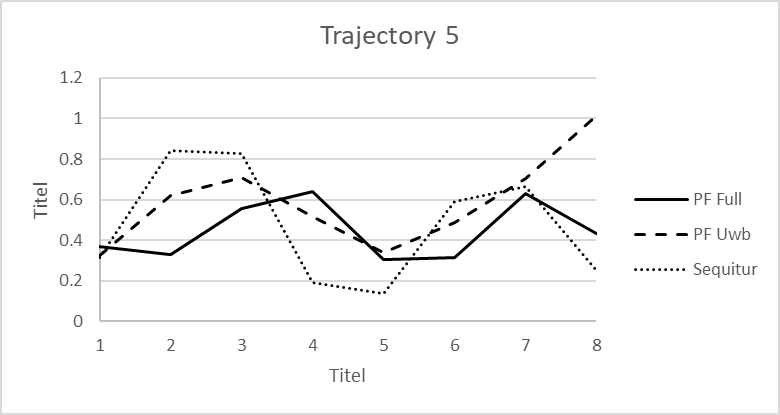
\includegraphics[width=0.8\textwidth]{Figures/trajectory5_results}
\decoRule
\caption[Positioning Results Trajectory 5]{Graph of measured distance errors at each checkpoint in trajectory 5.}
\label{fig:trajectory5_results}
\end{figure}

\begin{table}
\caption{The Arithmetic Mean of Errors in Trajectory 5 (meter).}
\label{tab:arithmetic_errors_trajectory5}
\centering
\begin{tabular}{l l l}
\toprule
\textbf{Trajectory} & \textbf{PF} & \textbf{Sequitur}\\
\midrule
\textbf{Total 1-4} & 1.73 & 1.93\\
\textbf{T5} & 0.49 & 0.48\\
\midrule
\textbf{Difference}  & \textbf{-1.24} & \textbf{-1.45}\\
\bottomrule\\
\end{tabular}
\end{table}
In Table \ref{tab:arithmetic_errors_trajectory5}, the mean errors of the low density AN scenario 1 and the high density AN scenario 2 are compared. The results improved significantly with a denser anchor node positioning. 
\begin{table}
\caption{Comparison of Scenario 1 and 2}
\label{tab:results_trajectory5}
\centering
\begin{tabular}{l l l l}
\toprule
\textbf{Algorithm} & \textbf{Mean error}[m] & \textbf{SD}[m] & \textbf{90\% Acc.}\\
\midrule
\textbf{PF (Scen 1)} & 1.729 & 1.451 & 3.393\\
\textbf{Sequitur (Scen 1)} & 1.928 & 2.337 & 5.544\\
\midrule
\textbf{PF (Scen 2)} & 0.491 & 0.239 & 0.875\\
\textbf{Sequitur (Scen 2)} & 0.484 & 0.271 & 0.829\\
\bottomrule\\
\end{tabular}
\end{table}
The standard deviation (SD) for scenario 2 was rather small with $0.24m$ for the PF and $0.27m$ for the Sequitur system, whereas the 90\% accuracy was $0.87m$ and $0.82m$. 
\begin{figure}[th]
\centering
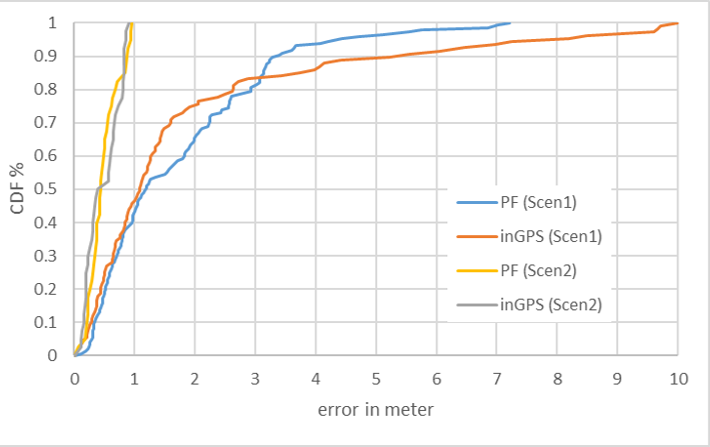
\includegraphics[width=0.8\textwidth]{Figures/cdf_all}
\decoRule
\caption[CDF Scenario 1 and 2]{The cummulative distribution function of the errors.}
\label{fig:cdf_all}
\end{figure}

\begin{figure}[th]
\centering
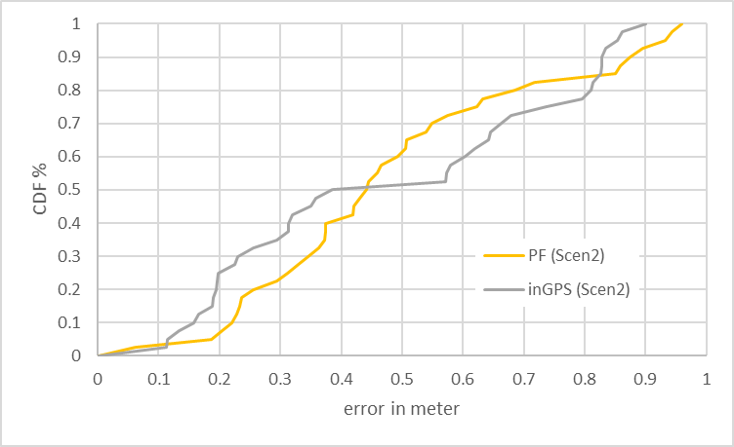
\includegraphics[width=0.8\textwidth]{Figures/cdf_scenario2}
\decoRule
\caption[CDF Scenario 2]{Zoomed cummulative distribution for scenario 2.}
\label{fig:cdf_scenario2}
\end{figure}
%----------------------------------------------------------------------------------------
%	SECTION 3
%----------------------------------------------------------------------------------------

\subsection{Result Analysis}
\label{Section2}
The test results in the experiment setup with wide anchor node distances were not very accurate. To find the reasons for that, we have to carefully have a look at the underlying implementation and the single checkpoint circumstances. We identified two main causes for bad results. These were:
\begin{itemize}
\item Some checkpoints were lying outside of AN bounding boxes.
\item UWB connection failed many times due to too wide distances from the TAG to the ANs
\end{itemize}
A cluttered environment will heavily distort UWB communication and thus affect the RTT used for UWB ranging. As in our testing environment servers with iron racks, desks with computer screens as well as a lot of different equipment was present. This effect should not be neglected.\\
\noindent\hspace*{5mm}%
The AN positions naturally form a bounding box around the environment. The bounding box is the area spanned by straight connections between anchor nodes, as indicated in Figure \ref{fig:trajectory1_boundingBox}. Trilateration, also with small distance errors, works well within the bounding box. However, even small ranging errors can lead to wrong position estimations outside the bounding box. 
\begin{figure}[th]
\centering
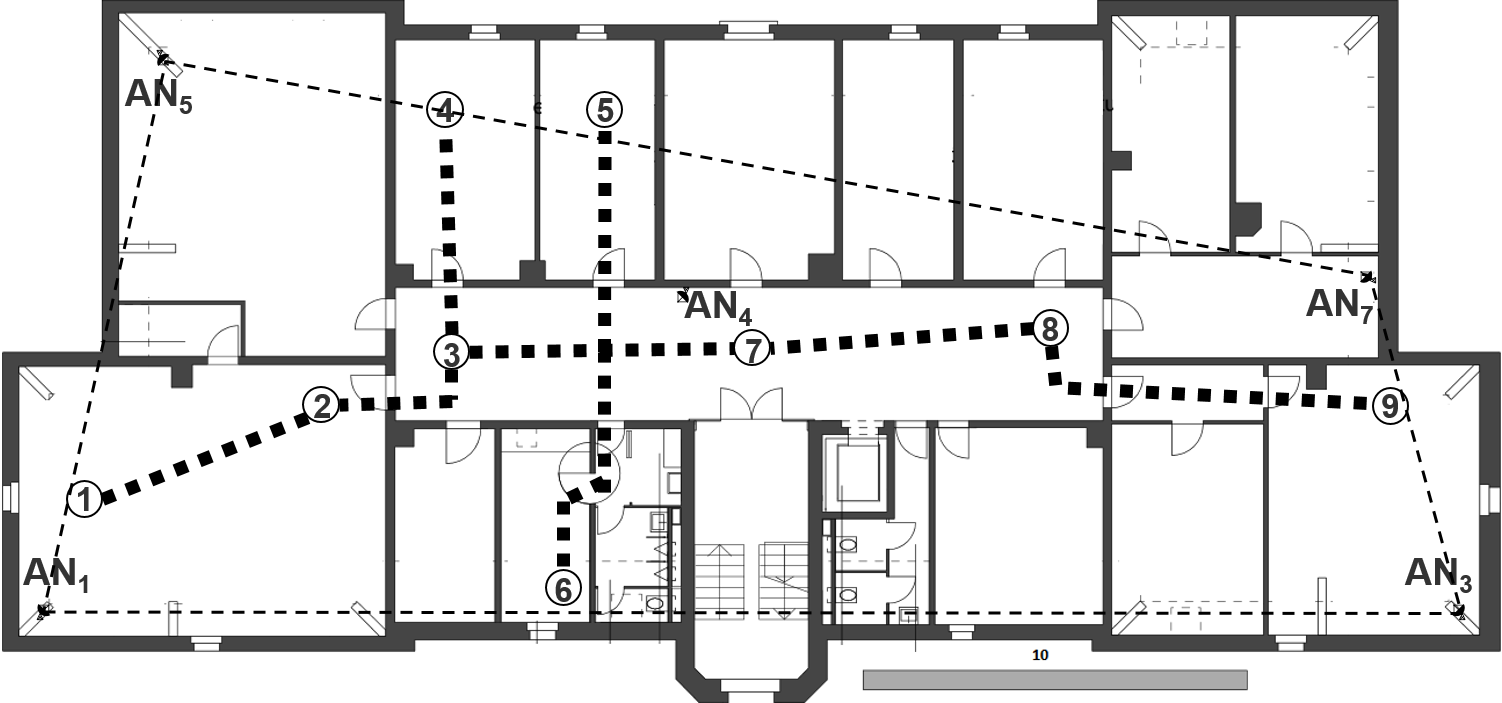
\includegraphics[width=0.8\textwidth]{Figures/trajectory1_boundingBox}
\decoRule
\caption[Bounding Box and Checkpoints for Trajectory 1 ]{Indicated bounding box of the anchor node positions for trajectory 1.}
\label{fig:trajectory1_boundingBox}
\end{figure}
In our experiment, especially the results on checkpoint 5 in trajectory 1 and 2 stand out. The average measured errors of $3.09m$ for PF and $5.70m$ for Sequitur for the first trajectory as well as $6.46m$ and $7.45m$ for the second trajectory are way higher than for other checkpoints. The fact that both algorithms had troubles estimating the position of checkpoint 5 in trajectory 1, leads to the conclusion that the experimental setup was the main reason for the big errors at this checkpoint. Moreover, besides lying outside the bounding box, this position was also far away from the nearest ANs without a direct line of sight.\\
\noindent\hspace*{5mm}%
Both algorithms depend on a well-established UWB connection, as all the ANs ranging estimations were transmitted using UWB messages. Especially in the particle filter, many UWB messages are transmitted, because fingerprinting and IMU data are additionally requested and exchanged. For certain checkpoints, the distance to the farthest anchor node was even more than $35m$ in scenario 1, which was too much for a stable UWB connection within our environment. Particularly, the particle filter had troubles receiving enough usable data, as it produced more overhead than the Sequitur system, because the particle filter transmitted IMU sensor data in addition to UWB ranging information. This led to a high packet loss, such that only one or two range measurements per estimation step were taken into account - instead of the possible five - leading to a higher error. \\
\noindent\hspace*{5mm}%
These surprisingly big inaccuracies of both systems prompted the change in our setup, in order to establish better communication between the nodes with less packet loss to enforce more data flowing into the particle filter. This was the main reason why we extended our experiments and evaluated the location accuracy in scenario 2.\\
\noindent\hspace*{5mm}%
With the more dense spread of the ANs, the estimations improved a lot. Having a look at our two assumptions above, we can state the following:

\begin{itemize}
\item Checkpoints outside of AN bounding boxes had quite a good accuracy, what contradicts our assumption.
\item The communication was better, what improved the accuracy a lot and confirmed our assumption.
\end{itemize}

In the new setup, we intentionally added checkpoints at the edge or outside of the bounding box, as seen in Figure \ref{fig:trajectory5_boundingBox}. Especially checkpoint 5 and 8 are not lying within the bounding box, however, they still had a quite good accuracy. For checkpoint 5, the average estimation errors were $0.30m$ and $0.14m$, for checkpoint 8 the errors were $0.43m$ and $0.25m$ for PF, respectively Sequitur.
\begin{figure}[th]
\centering
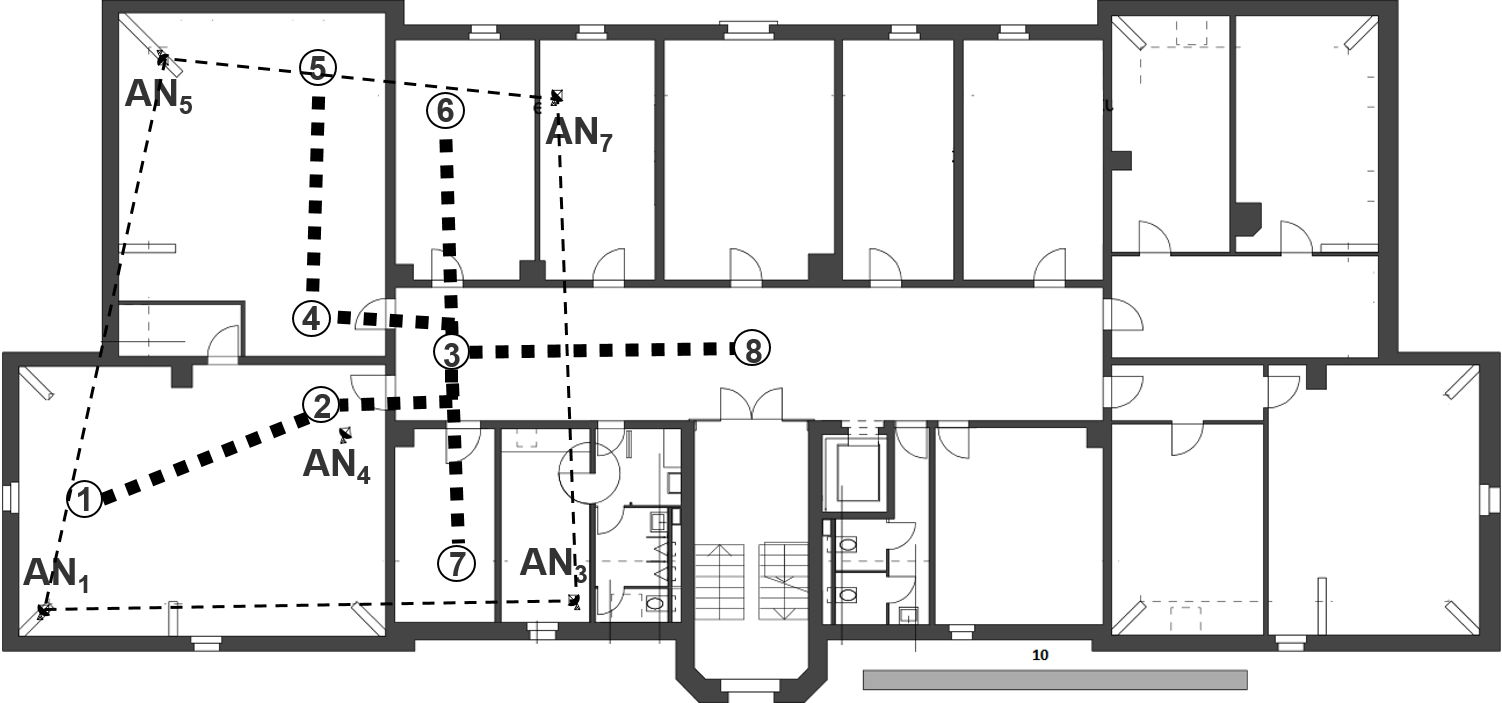
\includegraphics[width=0.8\textwidth]{Figures/trajectory5_boundingBox}
\decoRule
\caption[Trajectory 5 with Bounding Box]{Indicated bounding box of the anchor node positions for trajectory 5.}
\label{fig:trajectory5_boundingBox}
\end{figure}
It did not make a difference for the TAG being outside the bounding box or not. We conclude that it is not very important to stay within the bounding box, especially when good ranging data is available. However, when the measured ranges to the ANs contain big errors, the system is able to compensate those errors better when the TAG is within the bounding box. \\
\noindent\hspace*{5mm}%
The UWB connection had a bigger influence on the estimation error than the bounding box. With a better-established connection - in our case with nearer ANs - we had a lower packet loss. The result was, that in each estimation step, more data was available for the positioning algorithms. This led to a better accuracy.\\
For the particle filter, the communication to the ANs is very important, because the data is requested serially. Serial communication only allows a limited number of retransmissions and the communication timeouts have to be kept short. Packet loss affects the data quality, such that some evaluating steps had to be performed with fewer measurement values. Obviously, the lack of measurement values led to bad results, as the particle filter improves its estimation by fusing many different measurements, which is not possible when a part of the data is not present.
% Chapter Template

\chapter{Performance Evaluation} % Main chapter title

\label{Chapter6} % Change X to a consecutive number; for referencing this chapter elsewhere, use \ref{ChapterX}
In this section we explain the setup of our two experiment scenarios and we present the positioning results of our experiments in detail.

%----------------------------------------------------------------------------------------
%	SECTION 1
%----------------------------------------------------------------------------------------

\section{Experiment Setup}
We tested our implementation in two complex indoor scenarios with trajectories through numerous of rooms on one floor in a real building of the University of Bern. The first scenario used an area of $715m^2$ and the second scenario $358m^2$. We distributed the UWB anchor nodes over several rooms to cover the area of interest homogenously.
\begin{figure}[th]
\centering
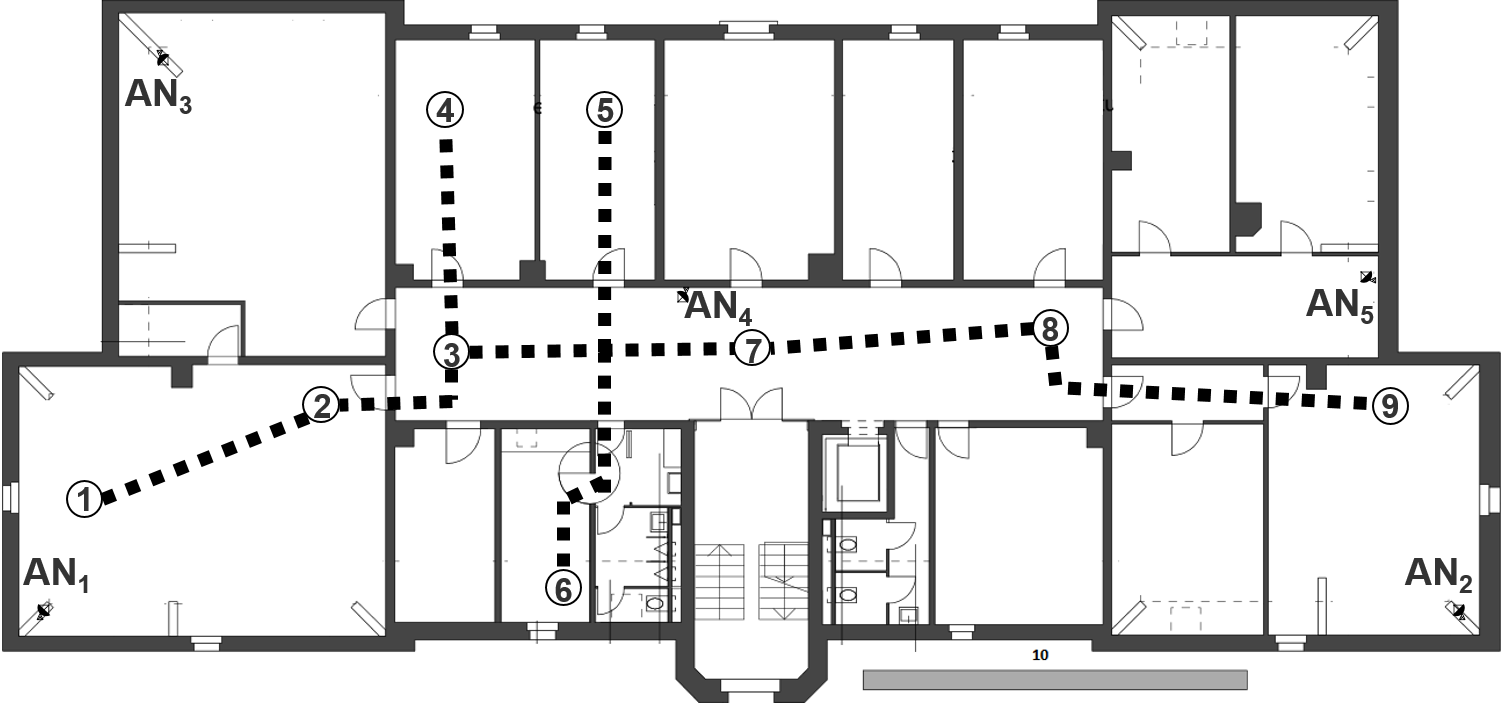
\includegraphics[width=0.8\textwidth]{Figures/trajectory1_withAnchors}
\decoRule
\caption[Anchor node positions]{Distributed anchor nodes on the floor map (with distance reference of 10m).}
\label{fig:trajectory1_withAnchors}
\end{figure}The exact position is indicated in the floor plan of figure \ref{fig:trajectory1_withAnchors} for the first scenario and indicated in figure \ref{fig:trajectory5_withAnchors} for the second scenario. In both scenarios the target was hold in the hand of a pedestrian at the starting point of the trajectories, when the experiments started. The pedestrian walked along the given trajectory path, as soon as he passed a predefined checkpoint the current position estimation was registered.\\
\noindent\hspace*{5mm}%
We defined four different trajectories for the first scenario. Each with five to nine checkpoints. Trajectory 1 is indicated in figure \ref{fig:trajectory1_withAnchors}, the other three trajectories can be seen in appendix \ref{AppendixA}.
For the second scenario we used a fifth trajectory that covered almost the whole area, it is shown in figure \ref{fig:trajectory5_withAnchors}.\\
\noindent\hspace*{5mm}%
We repeated the experiments five times, so we analized 145 checking points in scenario 1 and 40 checking points in scenario 2.\begin{figure}[th]
\centering
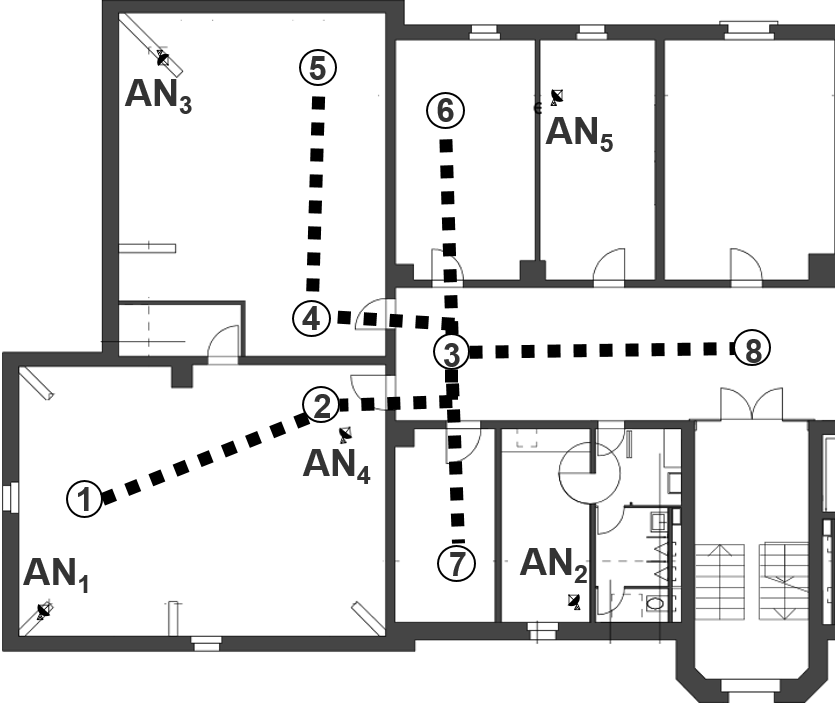
\includegraphics[width=0.5\textwidth]{Figures/trajectory5_withAnchors}
\decoRule
\caption[Trajectory 5]{Trajectory 5 with improved anchor positions.}
\label{fig:trajectory5_withAnchors}
\end{figure}
The localization error was determined by the euclidian distance between the systems position estimation and the real position of the checking point.\\
\noindent\hspace*{5mm}%
For the zone indication we defined 14 zones, which corresponded to 13 different rooms, where only one room was split in two zones. The room definitions can be seen in figure \ref{fig:zone_definition}. For scenario 1 we collected data in all zones, whereas for the smaller scenario we only collected data in the rooms 1, 2, 3, 5, 6 and 7, as only these were in the area of interest. The received signal strength of all five UWB ANs as well as of eight Wi-Fi access points was taken into account. The machine learning algorithms were fed with RSS difference to a given pivot RSS. The fourth AN and the neighboring WiFi access point were acting as pivot. In the offline phase of the fingerprinting, we collected around 700 fingerprint measures per room. Half of them were collected randomly passing the room and half of them was collected while systematically walking through the whole area of the room.
\begin{figure}[th]
\centering
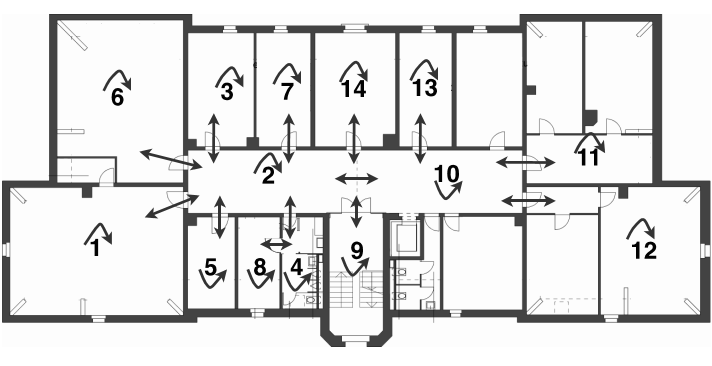
\includegraphics[width=1.0\textwidth]{Figures/zone_definition}
\decoRule
\caption[Zone definition]{Zone definition and transitions between zones}
\label{fig:zone_definition}
\end{figure}

\section{Experiment Results}
Experiments were first conducted in scenario 1, then we improved the anchor node position and conducted the experiments for scenario 2. As a reference we tested the same two scenarios with a different localization algorithm commercially proposed by UNISET Company, called Sequitur InGPS Lite. In the following we compare our particle filter results to the Sequitur system results.
\subsection{Positioning Results for Scenario 1}
In the following the results of our algorithms with a wide distance between anchor nodes (scenario 1) are shown. The results are shown as arithmetic means of the five probes we registered. In the first trajectory, the arithmetic mean (hereafter often called average) distance error over all checkpoints was $1.62$ meter for the particle filter and $1.75$ meter for Sequiturs commercial system. Looking at figure \ref{fig:trajectory1and2_results}, we see that the errors are often smaller than $1.5m$, however, there are some checkpoints with very low accuracy. This is also emphasized by comparing the arithmetic mean error to the median error of $1.12m$ for PF and $1.13m$ for Sequitur, which are significantly lower than the arithmetic means. The measurements for trajectory two were almost identical. The arithmetic mean error for the PF was $2.39m$ and for Sequitur $2.35m$. The median errors were again a lot more accurate with $1.59m$ for PF and $1.16m$ for Sequitur.
\begin{figure}[th]
\centering
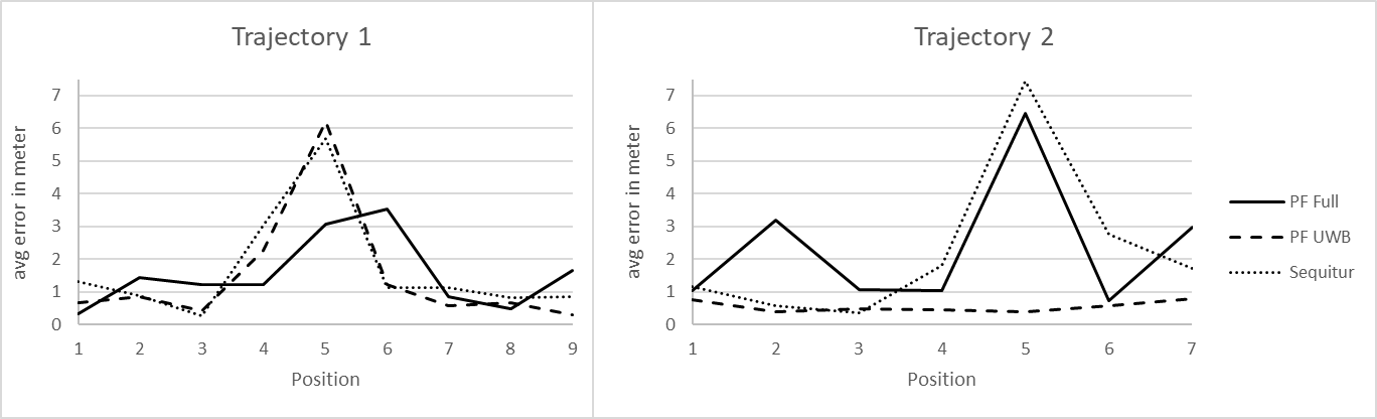
\includegraphics[width=1.0\textwidth]{Figures/trajectory1_2_results}
\decoRule
\caption[Positioning results trajectory 1 and 2]{Graphs of measured distance errors at each checkpoint in trajectory 1, respectively trajectory 2.}
\label{fig:trajectory1and2_results}
\end{figure}
The results for trajectory 3 and 4 were rather similar, however, the peaks observed in figure \ref{fig:trajectory3and4_results} were not as extreme as for the first two trajectories. As above, the average errors in the third trajectory of $1.23m$ (PF) and $1.94m$ (Sequitur) were also mentionable higher than the medians of $0.95m$ and $0.80m$.
\begin{figure}[th]
\centering
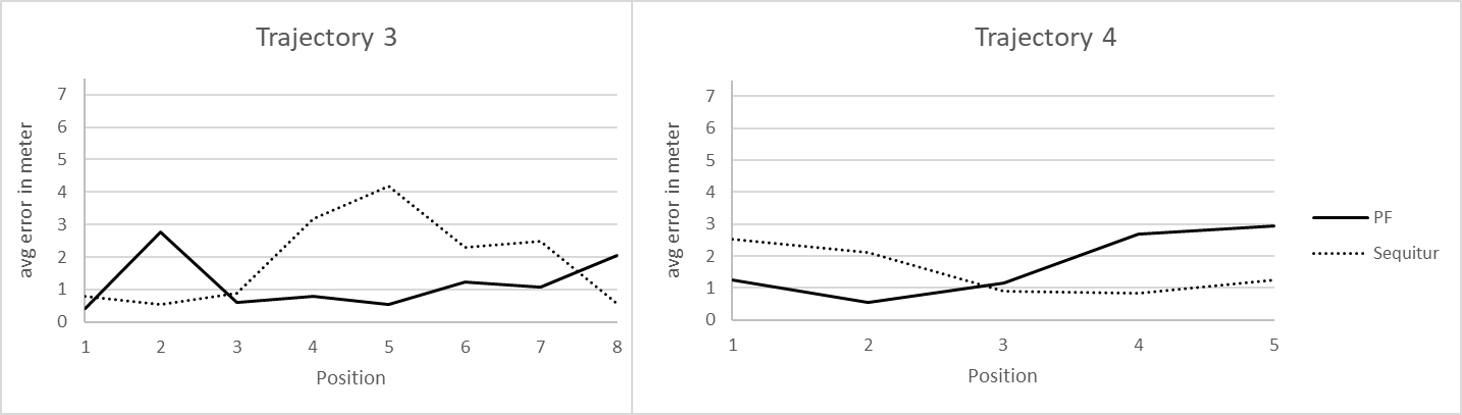
\includegraphics[width=1.0\textwidth]{Figures/trajectory3_4_results}
\decoRule
\caption[Positioning results trajectory 3 and 4]{Graphs of measured distance errors at each checkpoint in trajectory 3, respectively trajectory 4.}
\label{fig:trajectory3and4_results}
\end{figure}In the last of these four trajectories no big outliers were stated. Nonetheless the average errors of $1.79m$ and $1.55m$, as well as the median errors $1.24m$ and $1.26m$ for the PF and Sequitur, were still not as accurate as intended.\\
\noindent\hspace*{5mm}%
Having a closer look at table \ref{tab:arithmetic_errors}, we see that there are very big differences between different trajectories. The particle filter and the Sequitur system have similar accuracies, for some trajectories one of the algorithms is better, for other trajectories the other performs better. Possible reasons for these volatile results are discussed in the upcoming subsection  \ref{Section2} about result comments. 

\begin{table}
\caption{The arithmetic mean of errors in trajectory 1 to 4 (in meter).}
\label{tab:arithmetic_errors}
\centering
\begin{tabular}{l l l}
\toprule
\textbf{Trajectory} & \textbf{PF} & \textbf{Sequitur}\\
\midrule
\textbf{T1} & 1.72 & 1.75\\
\textbf{T2} & 2.39 & 2.35\\
\textbf{T3} & 1.23 & 1.94\\
\textbf{T4} & 1.79 & 1.55\\
\midrule
\textbf{Total 1-4}  & \textbf{1.73} & \textbf{1.93}\\
\bottomrule\\
\end{tabular}
\end{table}

%----------------------------------------------------------------------------------------
%	SECTION 2
%----------------------------------------------------------------------------------------

\subsection{Positioning Results for Scenario 2}
For trajectory 5 the distances between the anchor nodes were shortened. The exact setup was indicated above in figure \ref{fig:trajectory5_withAnchors}. Equally as before the results are shown as arithmetic means of the five test repetitions.\\
\noindent\hspace*{5mm}%
The results in this setup were way better than with wider ANs. With an average error of $0.49m$ for the PF and $0.48m$ for Sequitur, this setup outperformed the other trajectories with both algorithms. Even the median errors - with $0.44m$ and $0.48m$ -  were not much different, which means that there are no huge differences over the different checkpoints. This can also be seen in figure \ref{fig:trajectory5_results}, where most of the errors are smaller than $0.80m$.

\begin{figure}[th]
\centering
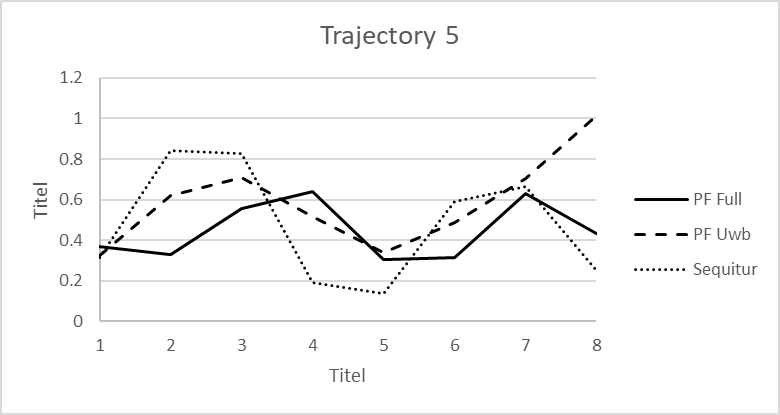
\includegraphics[width=0.8\textwidth]{Figures/trajectory5_results}
\decoRule
\caption[Positioning results trajectory 5]{Graphs of measured distance errors at each checkpoint in trajectory 5.}
\label{fig:trajectory5_results}
\end{figure}

\begin{table}
\caption{The arithmetic mean of errors in trajectory 5 (in meter).}
\label{tab:arithmetic_errors_trajectory5}
\centering
\begin{tabular}{l l l}
\toprule
\textbf{Trajectory} & \textbf{PF} & \textbf{Sequitur}\\
\midrule
\textbf{Total 1-4} & 1.73 & 1.93\\
\textbf{T5} & 0.49 & 0.48\\
\midrule
\textbf{Difference}  & \textbf{-1.24} & \textbf{-1.45}\\
\bottomrule\\
\end{tabular}
\end{table}
In table \ref{tab:arithmetic_errors_trajectory5}, the results of the low density AN scenario 1 and the high density AN scenario 2 are compared. The results improved significantly with a denser anchor node positioning. 
\begin{table}
\caption{Table of results for trajectory 5.}
\label{tab:results_trajectory5}
\centering
\begin{tabular}{l l l l}
\toprule
\textbf{Algorithm} & \textbf{Mean error}[m] & \textbf{S.D}[m] & \textbf{90\% Acc.}\\
\midrule
\textbf{PF (Scen 1)} & 1.729 & 1.451 & 3.393\\
\textbf{Sequitur (Scen 1)} & 1.928 & 2.337 & 5.544\\
\midrule
\textbf{PF (Scen 2)} & 0.491 & 0.239 & 0.875\\
\textbf{Sequitur (Scen 2)} & 0.484 & 0.271 & 0.829\\
\bottomrule\\
\end{tabular}
\end{table}
The standard deviation (S.D) for scenario 2 was rather small with $0.24m$ for the PF and $0.27m$ for the Sequitur system, whereas the 90\% accuracy was $0.87m$ and $0.82m$. 
\begin{figure}[th]
\centering
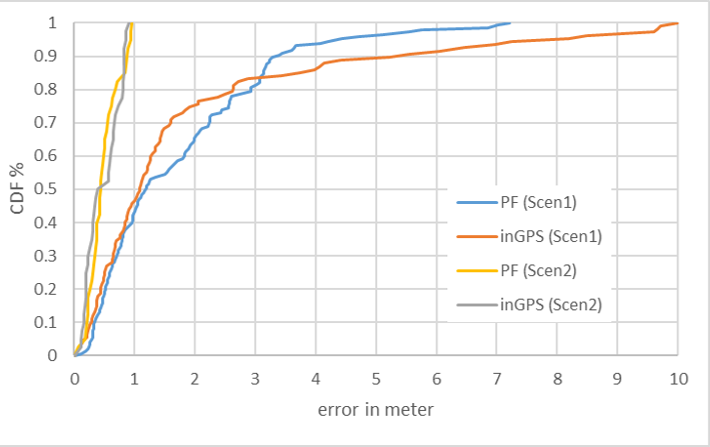
\includegraphics[width=1.0\textwidth]{Figures/cdf_all}
\decoRule
\caption[CDF]{The cummulative distribution function of the errors.}
\label{fig:cdf_all}
\end{figure}

\begin{figure}[th]
\centering
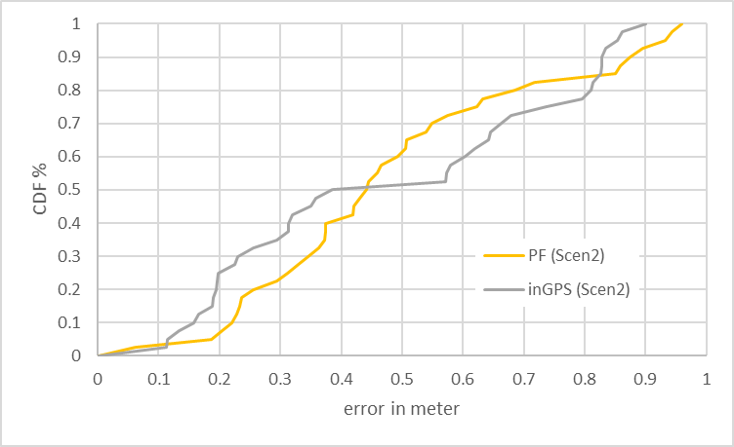
\includegraphics[width=1.0\textwidth]{Figures/cdf_scenario2}
\decoRule
\caption[CDF]{Zoomed cummulative distribution for scenario 2.}
\label{fig:cdf_scenario2}
\end{figure}
%----------------------------------------------------------------------------------------
%	SECTION 3
%----------------------------------------------------------------------------------------

\subsection{Comments on Test Results}
\label{Section2}
The test results in the experiment setup with wide anchor node distances were not as good as intended. To find the reasons for that, we have to carefully have a look at the underlying implementation and the single checkpoint circumstances. We identified two main causes for bad results, these were:
\begin{itemize}
\item Checkpoints outside of AN bounding boxes
\item Failing UWB connection due to too wide distances to ANs
\end{itemize}
A cluttered environment will heavily distort UWB communication and thus affect the RTT used for UWB ranging. As in our testing environment servers with iron racks, desks with computer screens as well as a lot of different equipment was present, this effect should not be neglected.\\
\noindent\hspace*{5mm}%
The AN positions naturally form a bounding box around the environment. The bounding box is the area spanned by straight connections between anchor nodes, as indicated in figure \ref{fig:trajectory1_boundingBox}. Trilateration, also with small distance errors, works well within the bounding box. However even small ranging errors can lead to wrong position estimations outside the bounding box. 
\begin{figure}[th]
\centering
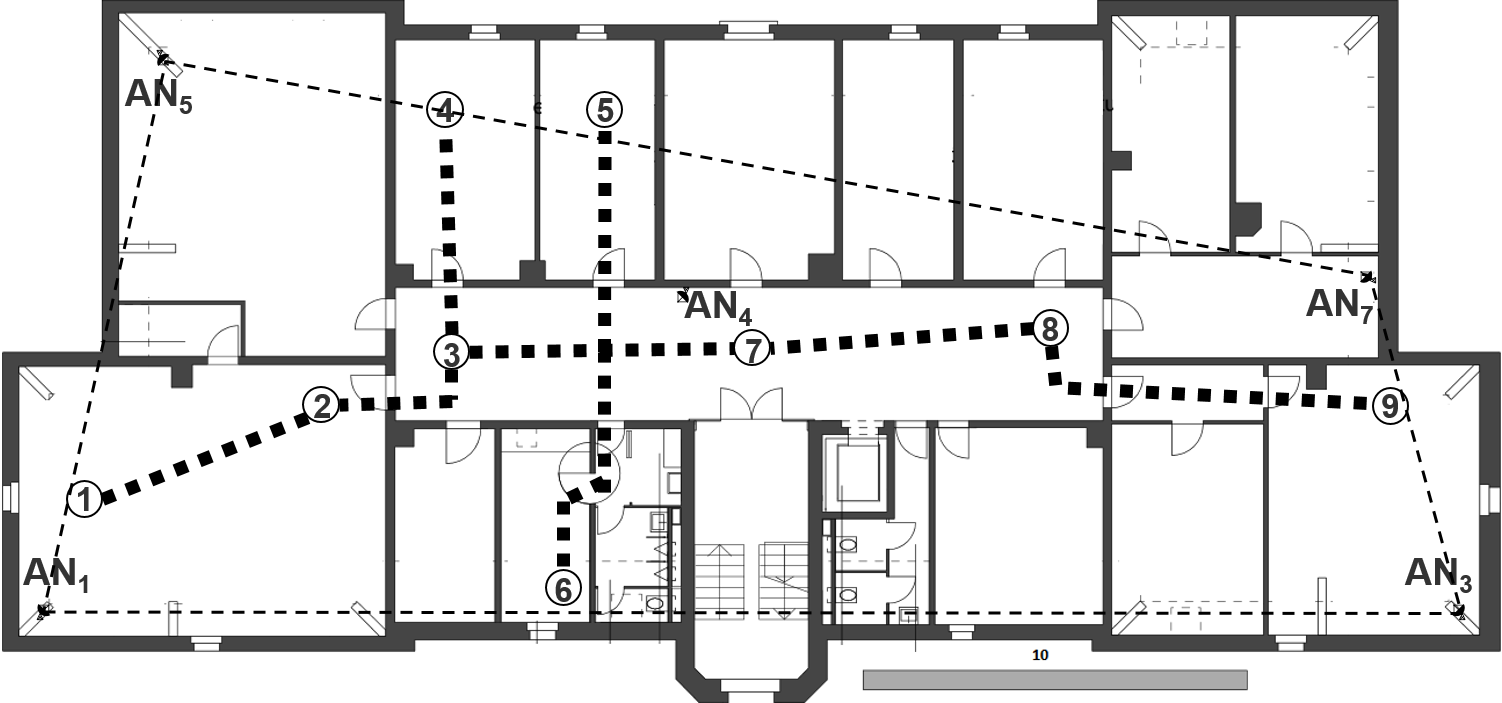
\includegraphics[width=0.8\textwidth]{Figures/trajectory1_boundingBox}
\decoRule
\caption[Bounding box and checkpoints for trajectory 1 ]{Indicated bounding box of the anchor node positions for trajectory 1.}
\label{fig:trajectory1_boundingBox}
\end{figure}
In our experiment especially the results on checkpoint 5 in trajectory 1 and 2 stand out. The average measured errors of $3.09m$ for PF and $5.70m$ for Sequitur during the first trajectory as well as $6.46m$ and $7.45m$ during the second trajectory are way higher than for other checkpoints. The fact that both algorithms had troubles estimating this position, leads to the conclusion that the experiment setup was the main reason for the big errors at this checkpoint. Moreover, not only lies this point outside the bounding box, but it was also far away from the nearest ANs without a direct line of sight.\\
\noindent\hspace*{5mm}%
Both algorithms depend on a good established UWB connection, as all the ANs ranging estimations are only transmitted via UWB. Especially in the particle filter many UWB meassages are transmitted, because fingerprinting and IMU data are additionally requested and exchanged. For certain checkpoints the distance to the farest anchor node was even more than $35m$ in scenario 1, which was too much for a stable UWB connection within our environment. Particularly, the particle filter had troubles receiving enough usable data, as it produced more overhead than the sequitur system. This led to a high package loss, such that only one or two range measurements per estimation step were taken into account - instead of the possible five - leading to a higher error. \\
\noindent\hspace*{5mm}%
These surprisingly big inaccuracies of both systems prompted the change in our setup, in order to establish better communication between the nodes with less package loss to enforce more data flowing into the particle filter. This was the main reason why we extended our experiments and evaluated the location accuracy in scenario 2.\\
\noindent\hspace*{5mm}%
With the more dense spread of the ANs, the estimations improved a lot. Having a look at our two assumptions above, we can state the following:

\begin{itemize}
\item Checkpoints outside of AN bounding boxes had quite good accuracy, adding doubts to this explanation.
\item The communication was better, what improved the accuracy a lot and confirmed our assumption.
\end{itemize}

In the new setup we purposely added checkpoints at the edge or outside the bounding box, as seen in figure \ref{fig:trajectory5_boundingBox}. Especially checkpoint 5 and 8 are not lying within the bounding box, however they still had a quite good accuracy. For checkpoint 5, the average estimation errors were $0.30m$ and $0.14m$, for checkpoint 8 the errors were $0.43m$ and $0.25m$ for PF, respectively Sequitur.
\begin{figure}[th]
\centering
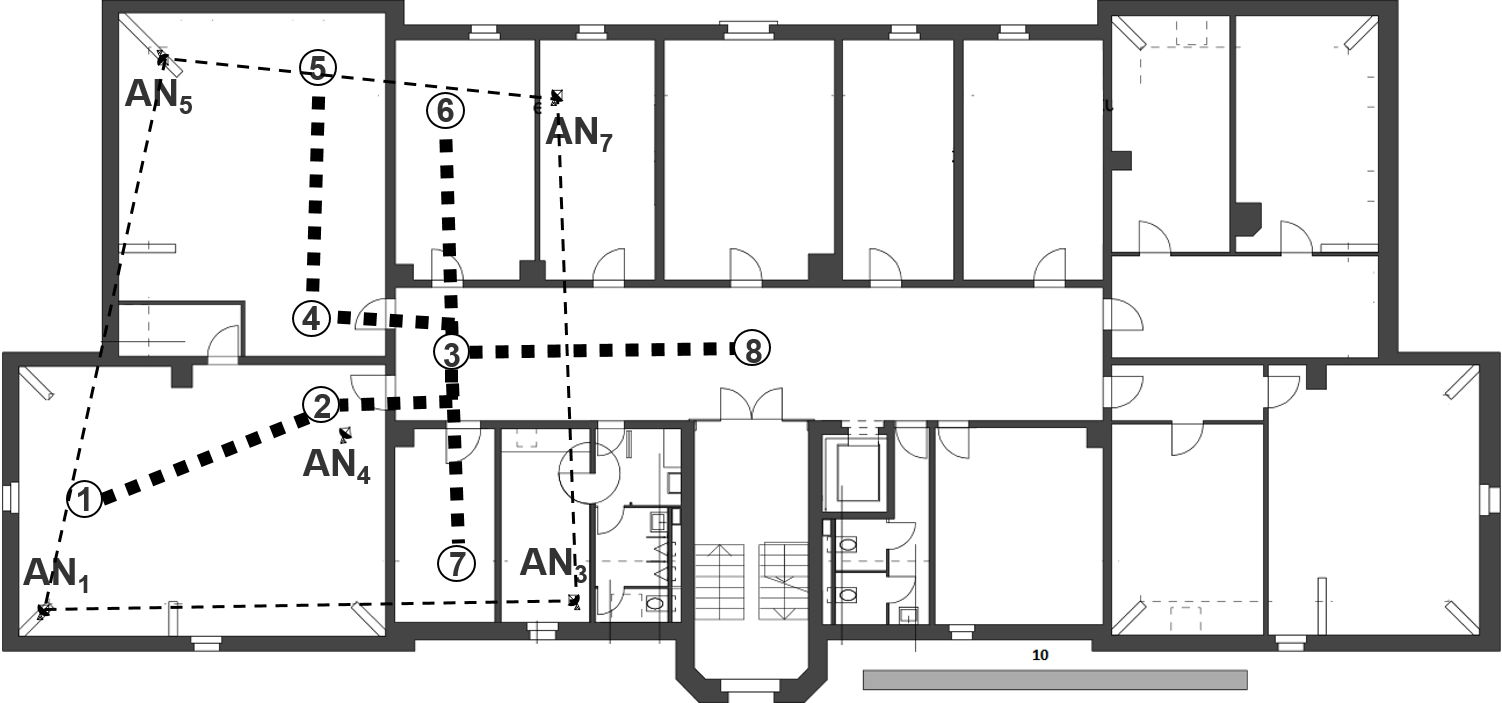
\includegraphics[width=0.8\textwidth]{Figures/trajectory5_boundingBox}
\decoRule
\caption[Trajectory 5 with bounding box]{Indicated bounding box of the anchor node positions for trajectory 5.}
\label{fig:trajectory5_boundingBox}
\end{figure}
It made no difference for the tag being outside the bounding box or not. We conclude that with good ranging data it is not very important to stay within the bounding box, however, wrong ranging data leads to bigger errors outside the bounding box.\\
\noindent\hspace*{5mm}%
A bigger influence on the estimation error had the UWB connection. With a better established connection - in our case with nearer ANs - more UWB messages arrived at the receiver. In each estimation step, more data was fed into the positioning algorithms what caused obviously a more precise performance. For the particle filter the communication is one of the key performance values, because the data is requested serially. This only allowes a limited amount of retransmitting and the communication timeouts have to be kept short. The resulting increased package loss affects the data quality, such that some evaluating steps had to be performed with less data. Obviously the lack of data led to bad results, as the particle filter improves its estimation by fusing many different measurements, what is not possible when a part of the data is not present.

%----------------------------------------------------------------------------------------
%	THESIS CONTENT - APPENDICES
%----------------------------------------------------------------------------------------

\appendix % Cue to tell LaTeX that the following "chapters" are Appendices

% Include the appendices of the thesis as separate files from the Appendices folder
% Uncomment the lines as you write the Appendices

% Appendix A

\chapter{Trajectories} % Main appendix title

\label{AppendixA} % For referencing this appendix elsewhere, use \ref{AppendixA}

\section{Figures of the trajectories used in the experiments}

\begin{figure}[th]
\centering
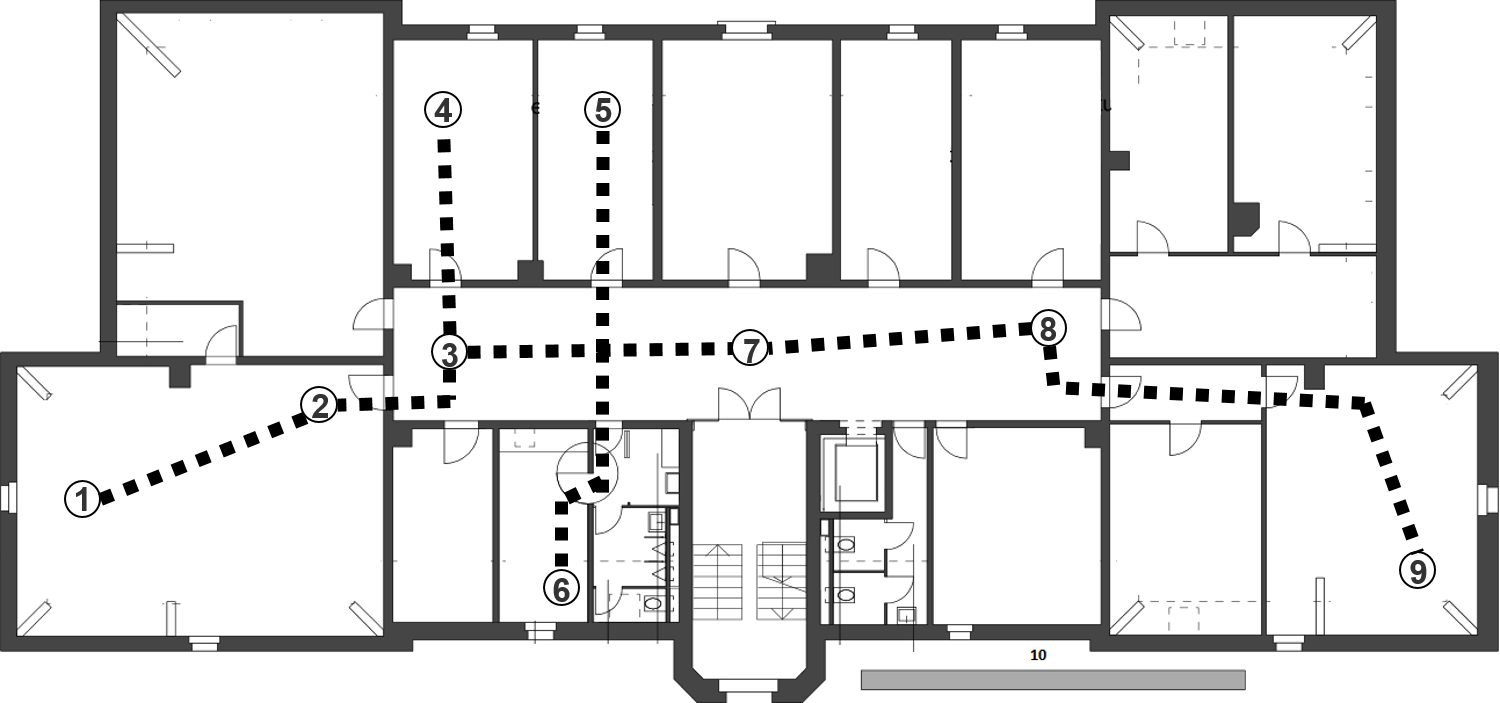
\includegraphics[width=1.0\textwidth]{Figures/trajectory1}
\decoRule
\caption[Trajectory 1]{Checkpoints and path of trajectory 1.}
\label{fig:trajectory1Appendix}
\end{figure}

\begin{figure}[th]
\centering
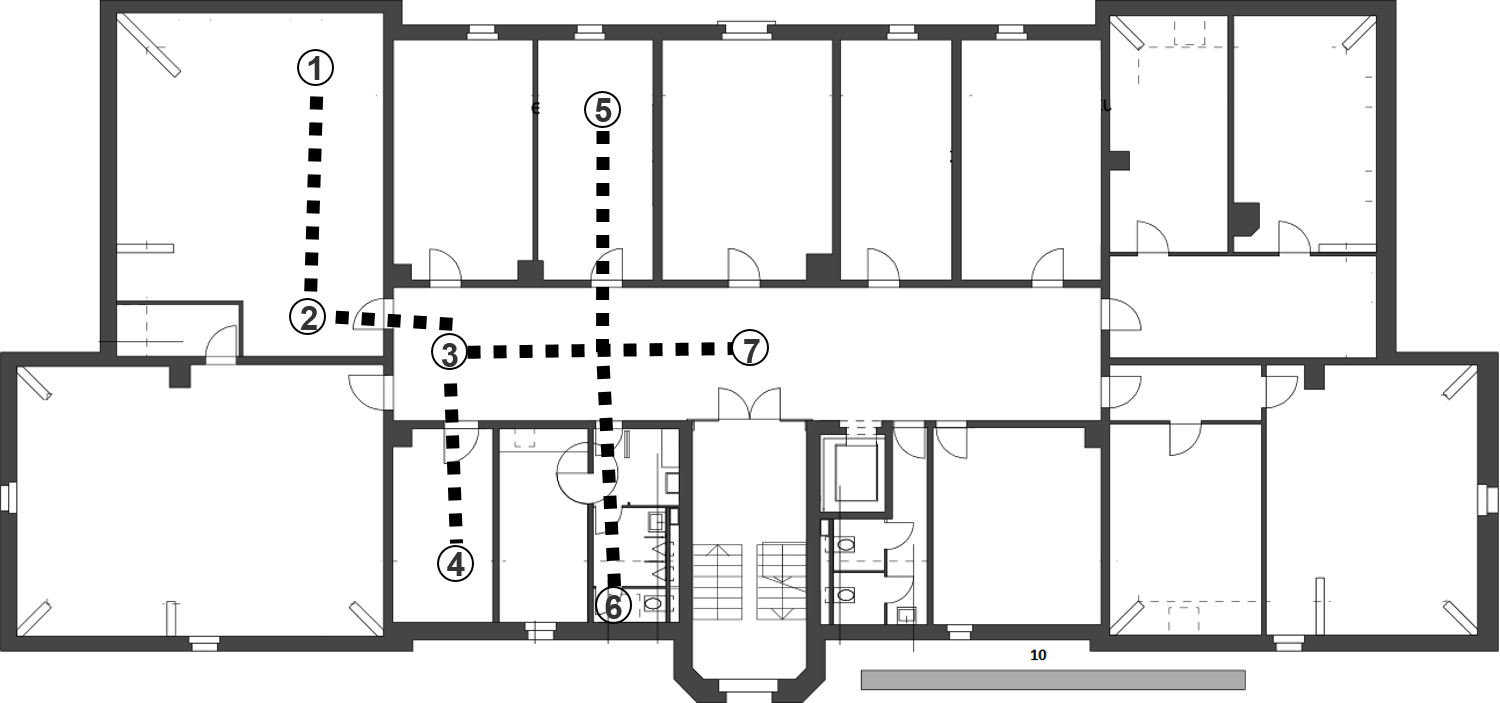
\includegraphics[width=1.0\textwidth]{Figures/trajectory2}
\decoRule
\caption[Trajectory 2]{Checkpoints and path of trajectory 2.}
\label{fig:trajectory2}
\end{figure}


\begin{figure}[th]
\centering
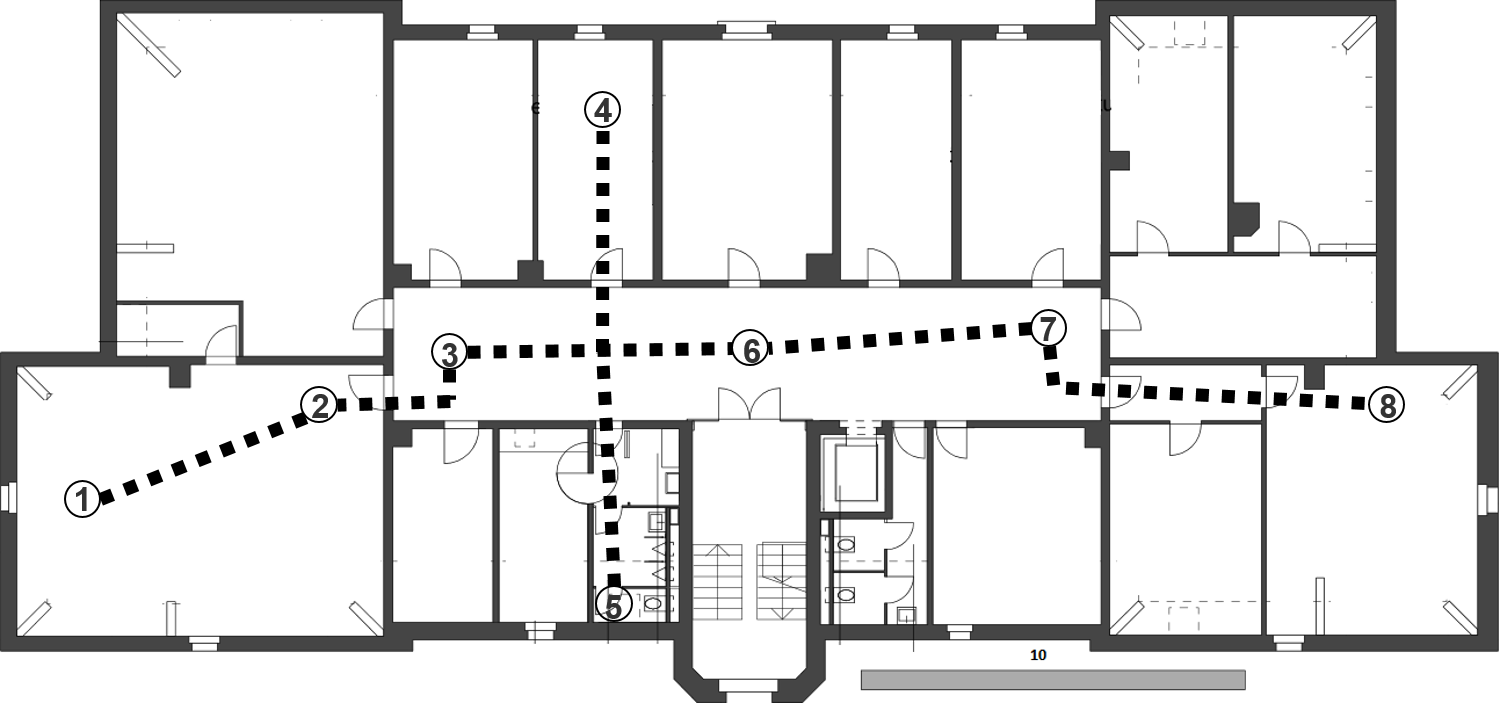
\includegraphics[width=1.0\textwidth]{Figures/trajectory3}
\decoRule
\caption[Trajectory 3]{Checkpoints and path of trajectory 3.}
\label{fig:trajectory3}
\end{figure}


\begin{figure}[th]
\centering
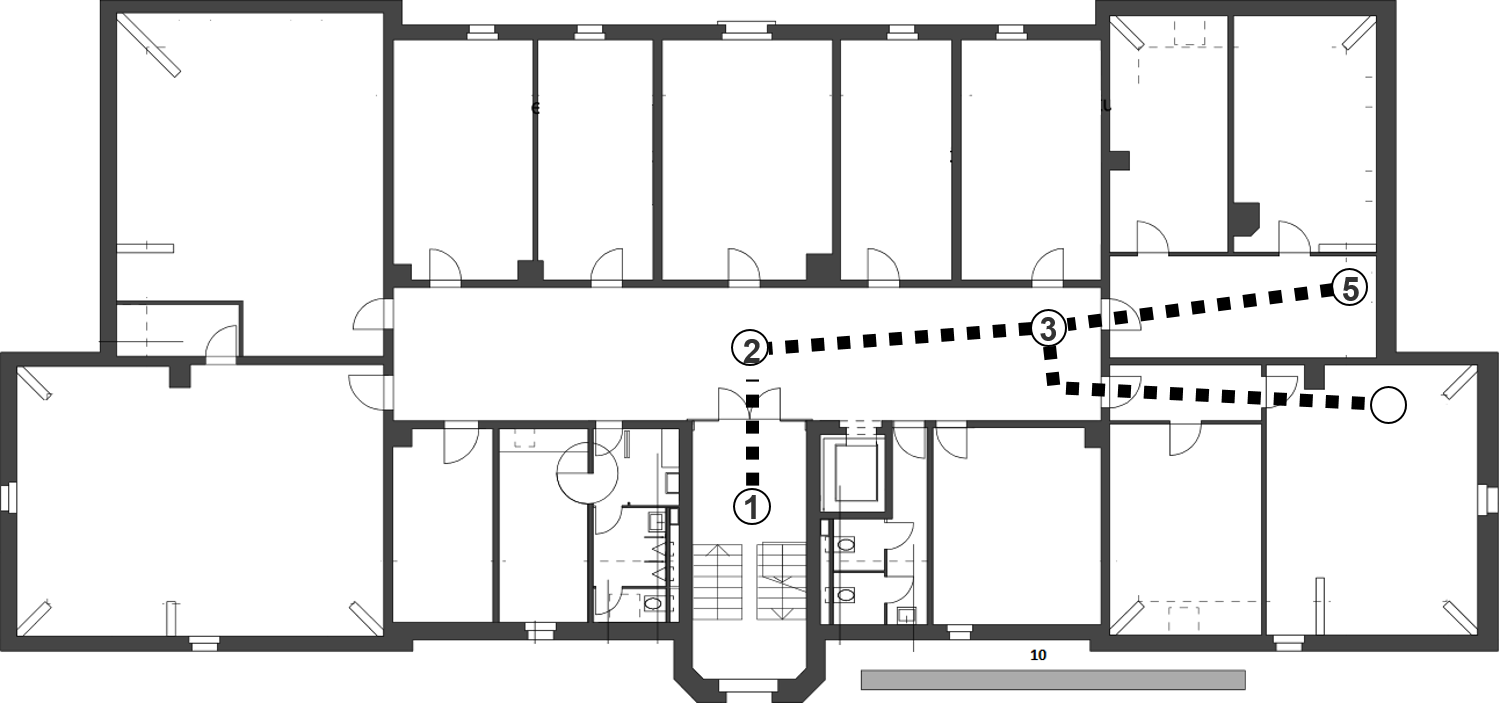
\includegraphics[width=1.0\textwidth]{Figures/trajectory4}
\decoRule
\caption[Trajectory 4]{Checkpoints and path of trajectory 4.}
\label{fig:trajectory4}
\end{figure}

%\include{Appendices/AppendixB}
%\include{Appendices/AppendixC}

%----------------------------------------------------------------------------------------
%	BIBLIOGRAPHY
%----------------------------------------------------------------------------------------

\printbibliography[heading=bibintoc]

%----------------------------------------------------------------------------------------

\end{document}  
